%\documentclass[jifs]{iosart2c}     
\documentclass[preprint,10pt,1p,twocolumns]{elsarticle}

%\documentclass[wias]{iosart2c}     

\usepackage[T1]{fontenc}
\usepackage{times}

\usepackage{fullpage}
\usepackage[ruled,vlined]{algorithm2e}

%%%%%%%%%%% Put your definitions here
%\usepackage[linesnumbered,ruled,vlined]{algorithm2e}% http://ctan.org/pkg/algorithms
%\usepackage{algpseudocode}% http://ctan.org/pkg/algorithmicx
\usepackage{amsthm}
\usepackage{amssymb,amsmath}
\usepackage{array,multirow}
\usepackage{amsfonts}

\usepackage{hyperref}
%\usepackage[linesnumbered,ruled,vlined]{algorithm2e}
\usepackage{epsfig}
\usepackage{float}
%\usepackage[lofdepth,lotdepth]{subfig}
\usepackage{float}
\usepackage{xcolor}
%\usepackage{mathptmx}
\usepackage{comment}
\usepackage{graphicx}
\usepackage{tabu}
%\usepackage{txfonts}
%\usepackage{subfigure}
\usepackage{color}
\usepackage{booktabs}
\usepackage{caption}
%\usepackage{subcaption}
\usepackage{url}
\usepackage{colortbl}
%\usepackage[sort&compress]{natbib}
\usepackage{lineno}
\usepackage{pdflscape}
\usepackage[inkscapelatex=false]{svg}
\usepackage{mathtools}
\usepackage{tikz}
\usetikzlibrary{positioning}
\usetikzlibrary{arrows.meta}
\usetikzlibrary{plotmarks}
\definecolor{lightgray}{rgb}{0.83, 0.83, 0.83}
\usepackage{pgfplots}
\pgfplotsset{
    axis background/.style={fill=lightgray},
    grid style={color=darkgray},
    tick label style={color=black},
    legend style={font=\small},
    label style={font=\small}
}
\usepackage{subcaption}
\newtheorem{deff}{Definition}
\newtheorem{prop}{Proposition}



%\usepackage[square, comma, numbers, sort&compress]{natbib}
%\setcitestyle{square, comma, numbers, sort&compress}
%%%%%%%%%%% End of definitions

%\pubyear{2020} 
%\volume{0}
%\firstpage{1}
%\lastpage{1}
\makeatletter
%\renewcommand{\arraystretch}{0.6}
\def\changemargin#1#2{\list{}{\rightmargin#2\leftmargin#1}\item[]}
\let\endchangemargin=\endlist 
\makeatother

\modulolinenumbers[5]

\newcommand{\changes}[1]{\textcolor{black}{#1}}
%\definecolor{ec}{rgb}{0.4, 0.26, 0.13}  % darkbrown
%\definecolor{ec}{rgb}{0.47, 0.27, 0.23} % bole
%\definecolor{ec}{rgb}{0, 0, 0} % black




%\journal{EJOR}

\begin{document}
\begin{frontmatter}   

\title{A Graph Neural Network Approach to Nanosatellite Task Scheduling: Insights into Learning Mixed-Integer Models}

\author[DAS]{Bruno Machado Pacheco} \ead{mpacheco.bruno@gmail.com }
\author[DAS,UNIVALI,PUC]{Laio Oriel Seman\corref{mycorrespondingauthor}} \ead{laio@univali.br}
\author[UFSC]{Cezar Antônio Rigo}\ead{cezar.a.rigo@gmail.com}
\author[DAS]{Eduardo Camponogara} \ead{eduardo.camponogara@ufsc.br}
%\author[MEC]{Edemar Morsch Filho} \ead{ede.morsch@gmail.com }
\author[UFSC]{Eduardo Augusto Bezerra} \ead{eduardo.bezerra@ufsc.br}
\author[UFPR,PUC]{Leandro dos Santos Coelho} \ead{leandro.coelho@pucpr.br}
%\author[UFSCar]{Pedro Augusto Munari Junior} \ead{munari@dep.ufscar.br}

%\runningauthor{}

\cortext[mycorrespondingauthor]{Corresponding author. E-mail: laio@univali.br}

\address[DAS]{Department of Automation and Systems Engineering, Federal University of Santa Catarina (UFSC), Florianópolis, Brazil}
\address[UNIVALI]{Graduate Program in Applied Computer Science, University of Vale do Itajaí (UNIVALI), Itajaí, Brazil}
\address[UFSC]{Department of Electrical Engineering, Federal University of Santa Catarina (UFSC), Florianópolis, Brazil}
\address[UFPR]{Department of Electrical Engineering, Federal University of Parana, Curitiba, Brazil}
\address[PUC]{Industrial and Systems Engineering Graduate Program, Pontifical Catholic University of Parana, Curitiba, Brazil}
%\address[MEC]{Department of Mechanical Engineering, Federal University of Santa Catarina (UFSC), Florianópolis, Brazil}
%\address[UFSCar]{Department of Production Engineering, Federal University of São Carlos (UFSCar), São Carlos, Brazil}

\begin{abstract}
This study investigates how to schedule nanosatellite tasks more efficiently using Graph Neural Networks (GNN). In the Offline Nanosatellite Task Scheduling (ONTS) problem, the goal is to find the optimal schedule for tasks to be carried out in orbit while taking into account Quality-of-Service (QoS) considerations such as priority, minimum and maximum activation events, execution time-frames, periods, and execution windows, as well as constraints on the satellite's power resources and the complexity of energy harvesting and management. The ONTS problem has been approached using conventional mathematical formulations and precise methods, but their applicability to challenging cases of the problem is limited. This study examines the use of GNNs in this context, which has been effectively applied to many optimization problems, including traveling salesman problems, scheduling problems, and facility placement problems. Here, we fully represent MILP instances of the ONTS problem in bipartite graphs. We apply a feature aggregation and message-passing methodology allied to a ReLU activation function to learn using a classic deep learning model, obtaining an optimal set of parameters. Furthermore, we apply Explainable AI (XAI), another emerging field of research, to determine which features -- nodes, constraints -- had the most significant impact on learning performance, shedding light on the inner workings and decision process of such models. We also explored an early fixing approach, obtaining an accuracy above 80\% both in predicting the feasibility of a solution and the probability of a decision variable value being in the optimal solution. Our results point to GNNs as a potentially effective method for scheduling nanosatellite tasks and shed light on the advantages of explainable machine learning models for challenging combinatorial optimization problems.
\end{abstract}



\begin{keyword}
Scheduling \sep Graph Neural Network \sep Combinatorial Optimization \sep  Nanosatellite \sep Quality of Service.
\end{keyword}

%\maketitle
\end{frontmatter}

%%%%%%%%%%% The article body starts:

\allowdisplaybreaks

\section{Introduction}
\label{sec:intro}
\begin{figure}[t]
\begin{center}
    \includegraphics[width=1\linewidth]{figures/teaser.pdf}
\end{center}
\vspace{-0.1in}
\caption{\textbf{{\em Foggy} vs {\em Clear} NeRF.} Our \ournerf gets rid of reconstruction errors manifested as foggy ``floaters" in the density volume without additional input or significant computational overhead. 
%
Below are density profiles along a given ray before and after our geometry correction procedure, where we discard density peaks corresponding to floaters.
}
\label{fig:teaser}
\vspace{-0.2in}
\end{figure}



%The emergence of 
Neural Radiance Fields (NeRFs)~\cite{mildenhall2020nerf}  %and its variants 
have made revolutionary contributions in %photo-realistic 
novel view synthesis~\cite{barron2021mip,barron2022mip}, 
autonomous driving~\cite{rematas2022urban,tancik2022block}, digital human~\cite{hong2022headnerf,zhao2022humannerf}, and 3D content generation~\cite{eg3d,poole2022dreamfusion,lin2022magic3d}.
%by leveraging a multi-layer perceptron (MLP) to implicitly model the mapping from input 5D coordinates (i.e., 3D coordinates $\mathbf{x} = (x,y,z)$ and 2D viewing directions $\mathbf{d}=(\theta,\phi)$) to volume density $\sigma$ and view-dependent emitted radiance color $\mathbf{c} = (r,g,b)$. 
%
%They then use traditional volume rendering mechanisms on the obtained continuous 5D function (i.e., MLP) to generate novel views. 
To date, unfortunately, most NeRF-based methods encounter challenges when tackling large-scale cluttered scenes (e.g., Fig.~\ref{fig:teaser}):
\begin{enumerate}[leftmargin=0.16in, topsep=2pt,itemsep=-1ex,partopsep=1ex,parsep=1ex]
\item Input observations used for NeRF are often too sparse  compared to forward-facing or synthetic looking-inward scenes;
%\item Recovering fine-grained objects within a large volume is challenging for NeRF; %in capturing details accurately.
\item View-dependent visual effects give rise to ambiguity, resulting in a ``foggy" density field as shown in Fig.~\ref{fig:teaser}. 
%
Such artifacts are particularly pronounced in indoor scenes strewn with view-dependent appearances, such as specular highlights, glossy surface reflections from man-made objects. 
\end{enumerate}

Despite attempts to enhance NeRF's rendering quality given suboptimal input, such as using 3D conical frustums~\cite{barron2021mip,barron2022mip}, physically-grounded augmentations~\cite{chen2022aug}, and misalignment correction~\cite{jiang2022alignerf},  these challenges have yet to be fully resolved.
%
Depth supervision~\cite{deng2022depth, wei2021nerfingmvs} or proxy geometry~\cite{xu2021scalable,wu2022scalable} images can help alleviate the challenges in handling large-scale with sparse input, at the expense of %but they come at the cost of requiring 
expensive pre-processing or additional input.
%
Another line of work~\cite{wang2021neus, oechsle2021unisurf, wang2022neuris} achieves better reconstruction of surface geometry by using signed distances instead of volume density as scene representation. However, they sacrifice the ability to synthesize photo-realistic novel views.

%We observe that NeRF has been suffering from foggy ``floater" artifacts in large-scale cluttered scenes.
%
%Such artifacts are particularly pronounced in indoor scenes strewn with view-dependent appearances from man-made objects. 
%
To address the above issues, we propose an extension to NeRF, dubbed as {\bf \ournerf}, which enforces effective {\em appearance} and {\em geometry} constraints conducive to accurate colors and 3D densities estimation. We believe \ournerf can contribute beyond novel view synthesis, such as NeRF object detection~\cite{hu2022nerf}, NeRF object segmentation~\cite{zhi2021place, liu2022unsupervised, fan2022nerf,ren2022neural}, and NeRF registration~\cite{goli2022nerf2nerf}, where the rooms for improvement are substantial if more accurate color and density estimation are available.

Correspondingly, there are two steps in \ournerf. First, for appearance correction, the view-independent and view-dependent color components are predicted from the underlying 3D scene, which is combined to produce the final color estimation (Fig.~\ref{fig:toaster}).
%
The view-independent component (diffuse color and shading) captures the overall scene color, while the view-dependent component (highlights or reflections) captures color variations due to changes in viewing angle.
%
\ournerf then discards these view-dependent appearances in the training views to prevent them from interfering with the density estimation.
%
Second, a simple and effective geometry correction procedure will be performed to further eliminate the foggy ``floaters" or density errors. This geometry correction procedure is based on an assumption in line with traditional ray tracing in computer graphics.
\begin{comment}
% xh: basically copying method
On the other hand, ClearNeRF performs a geometric correction procedure performed on each traced ray during inference to refine the density estimation and better tackle the floater artifacts. 
%
The geometry correction procedure assumes that there should only be one salient peak along each traced ray during NeRF inference. 
Only the salient peak closest to the ray origin (the camera center) corresponds to  true geometry while the others will be manifested as foggy floaters hovering in the density volume. 
%
This assumption is in line with traditional ray tracing in computer graphics where in the absence of noise, only one intersection per ray should be returned to indicate the closest ray-object intersection.
%
\end{comment}
%%%%%%%%%%%
%As shown in Fig.~\ref{fig:teaser}, when reconstructing an indoor scene with sparse input and highly view-dependent objects, NeRF produces severe floating artifacts due to its attempt to explain view-dependent appearances.
%
Experiments verify that our proposed \ournerf can effectively get rid of floater artifacts without additional input.% or significant computational overhead. 


In summary, our contributions include the following:
\begin{itemize}[leftmargin=0.16in, topsep=2pt,itemsep=-1ex,partopsep=1ex,parsep=1ex]
    \item We propose a concise method for decomposing view-independent and view-dependent appearance during NeRF training and eliminate the interference of view-dependent appearance.
    \item We propose a geometric correction procedure performed on each traced ray during inference to refine the density estimation and better tackle the floater artifacts.
    \item Extensive experiments and ablations verify the effectiveness of our core designs and results in improvements over the vanilla NeRF and other state-of-the-art alternatives.
    %without additional computational resources or other inputs.
\end{itemize}




\section{Related Works}

\begin{figure*}[!ht]
\centering
\includegraphics[width=\linewidth]{body/figures/data_collection2.png}
\caption{\textbf{Hardware Setup.} We use a GelSight Wedge sensor for tactile sensing, an Intel ReslSense D405 camera mounted on the side for RGB vision sensing, and an OptiTrack setup for motion capture. \textbf{Data Collection.} The tactile finger and the camera are fixed to the table at all times. A human operator moves a test object and presses it against the finger. We show sampled tactile and RGB images as well as a reconstructed local tactile depth map on the right.}
\label{datacollection}
\end{figure*}

% \textbf{Tactile sensors}:
% Over the years, researchers have developed tactile sensors working on different sensing principles, such as resistance, capacitance, magnetic, barometric, and optic.
% We refer readers to \cite{kappassov2015tactile} for an in-depth review of different types of tactile sensors and their applications.
% Compared to other sensing principles, GelSight tactile sensors have the advantage of providing high-resolution geometrical information of the contact surface.
% They are usually constructed with an elastic silicone gel, directional colored LEDs, and a camera pointing at the gel.
% The gels are usually coated with reflective paint with printed dots.
% When in contact, the gel deforms and takes the shape of the contact surface.
% Shear force can be retrieved by tracking dot movements.
% Furthermore, the color value of a pixel is correlated with the gradient of the height of the contact surface at the specific location. 
% With a pre-calibrated color table, a depth map can be reconstructed from the color image.
% This type of tactile sensor is selected for our work for its rich output and ease to use.

Researchers of the robotics community have put forward a wide range of tactile sensing solutions.
Sensors working on different sensing principles have been adopted to solve a large set of manipulation tasks.
Among different types of tactile sensors, vision-based ones such as GelSight \cite{yuan2017gelsight} and GelSlim \cite{donlon2018gelslim} stand out for their rich output, ease to use, and affordability.
While we focus on the pose estimation and shape reconstruction task using vision-based tactile sensors, we refer readers to \cite{kappassov2015tactile} for an in-depth review of different types of tactile sensing and their applications.
In this section, we review works on three typical tasks that are most relevant to our solution: slip detection, object property inference, and SLAM.

% Researchers have found that using this class of vision-based tactile sensors can greatly increase the accuracy when reasoning about the contact surface, compared to traditional tactile sensors that are constructed with normal direction force sensors [\todo{add citation}].

\textbf{Slip detection and estimation}:
Using a similar sensor to ours, Yuan \etal compared and analyzed a GelSight tactile sensor's images collected at different stages of slip in \cite{yuan2015measurement} and showed this type of sensors' capability in detecting micro scale movements.
Li \etal and Zhang \etal trained recurrent neural networks on tactile images to detect slip between multiple time steps in a manipulation sequence \cite{li2018slip, zhang2018fingervision}.
Built on their binary slip detection model in \cite{li2018slip}, Li further added rotational slip direction prediction in \cite{li2019rotational}.
Calandra \etal improved a grasp planner for the classic robot bin-picking problem by incorporating slip detection and achieved a higher grasp success rate \cite{calandra2017feeling}. 
However, those methods only detect slip without localizing the object after the slip.
In many precision manipulation tasks we are also interested in the amount of the displacement.

\textbf{Object property inference and localization}:
% With detailed information on the contact surface provided by high-resolution tactile sensors, 
Many works have focused on inferring properties of the in-contact object, such as shape \cite{strub2014using, luo2015tactile, luo2019iclap}, texture \cite{luo2018vitac, yuan2017connecting}, and material \cite{yuan2017connecting, kroemer2011learning, kerr2018material}.
Those learned object properties can be further used for localization.
In order to localize current grasps, Bauza \etal proposed to match new tactile imprints with previously collected tactile imprints \cite{bauza2019tactile}, while Luo \etal learned to match tactile imprints directly to visual images of the whole object \cite{luo2015localizing}.
Assuming known CAD models, Bauza \etal proposed to localize by comparing contact masks generated from tactile images with a large bank of random projections of the CAD model \cite{bauza2022tac2pose}.
To solve the reverse problem, i.e. what a tactile image looks like given an object and a pose, several tactile simulators have been built to automatically generate tactile images given an object's CAD model and a finger pose \cite{si2022taxim, wang2022tacto}.
One major limitation for this category of works is that they all require a known calibrated geometry of the object: a pre-collected tactile map \cite{bauza2019tactile}, a model of the object \cite{bauza2022tac2pose}, or a global image with known geometry \cite{luo2015localizing}.
This requirement can be hard to meet in less constraint environments.

\textbf{Tactile SLAM}:
Recent studies have shown interests in working with unknown objects by leveraging methods from the SLAM problem.
With a focus on 2D shapes, Suresh \etal parameterized shapes as Gaussian Process Implicit Surfaces (GPIS), and learned its parameters from tactile signals collected during pushing \cite{suresh2021tactile}.
Assuming known contact poses, authors of \cite{suresh2022shapemap} first learned a noisy mapping from known surface geometries to corresponding tactile images, then reconstructed an object by combining many noisy local tactile measurements into an optimized global shape using factor graph optimization.
The closest prior work to ours is \cite{sodhi2022patchgraph}, where the authors learned to estimate 6D poses and 3D shapes simultaneously for unknown objects. 
They constructed a pose estimator based on tactile sensing, and a shape reconstruction pipeline that added in new tactile point clouds incrementally on the run.
However, this approach heavily relies on the performance of the tactile pose estimator, which lacks a global understanding of the object and can suffer from repeated patterns or smooth surfaces.
In contrast, our work combines vision and tactile sensing which provides us with both global and local understandings of the scene without requiring any other domain knowledge.
Furthermore, we designed a loop closure mechanism that periodically matches current tactile and vision images to stored key-frames, which significantly reduced accumulated errors.
With this, FingerSLAM is able to produce realistic reconstructions even in long sequences. 
\section{Problem Statement}\label{sec:problem}

Given a set of jobs $\mathcal{J}=\{0,...,J\}$ that represent a mission and a set of time units $\mathcal{T}=\{0,...,T\}$ that represents the orbit period, the objective function \eqref{objetivo} represents the goal of maximizing the mission quality of service (QoS) metric, which is represented as the sum of the priority values $u_{j,t}$ for all the jobs $j$ over all the periods $t$.
\begin{align} \label{objetivo}
QoS :~~
	\underset{x_{j,t}}{\max} ~~
	\underbrace{\sum_{j=1}^{J} \sum_{t=1}^{T} {u}_{j,t} x_{j,t} }_{ \text{Quality of Service}}
% x_{j,t}\in\{0,1\}, ~~\quad \forall j\in\mathcal{J}, t\in\mathcal{T} 
\end{align}
Variable $x_{jt}$ represents the binary decision of scheduling job $j$ at time $t$, which takes on value $1$ if job $j$ is scheduled to run at time $t$ and $0$ otherwise.

In constraints \eqref{phiA} to \eqref{phiE}, the variable $\phi_{j,t}$ is used to describe the period between task executions. In essence, these equations enforce the relationship between $\phi_{j,t}$ and $x_{j,t}$ such that $\phi_{j,t}$ assumes value 1 only in the time step the task $j$ started running and is later used to reflect the desired period between task executions in the scheduling problem.
%
\begin{subequations} \label{qos_constraints}
    \begin{align}
        &\phi_{j,t} \geq x_{j,t}, &~\forall j\in\mathcal{J},\, t = 1 \label{phiA} \\
        %%%%%%%%%%%%%%%%%%%%%%%%%%%%%%%%%%%%%%%%%%%%%%%%%%%%%%%%%%%%%%%%%%%%%%%%%%%%%%%%%%%%%%%%%%%%%%%%%%%
        &\phi_{j,t} \geq x_{j,t} - x_{j,(t-1)}, &~\forall j\in\mathcal{J}, \,\forall t\in\mathcal{T}: t > 1  \label{phiB} \\
        %%%%%%%%%%%%%%%%%%%%%%%%%%%%%%%%%%%%%%%%%%%%%%%%%%%%%%%%%%%%%%%%%%%%%%%%%%%%%%%%%%%%%%%%%%%%%%%%%%%
        &\phi_{j,t} \leq x_{j,t}, &~\forall j\in\mathcal{J}, \,\forall t\in\mathcal{T}  \label{phiC} \\
        %%%%%%%%%%%%%%%%%%%%%%%%%%%%%%%%%%%%%%%%%%%%%%%%%%%%%%%%%%%%%%%%%%%%%%%%%%%%%%%%%%%%%%%%%%%%%%%%%%%
        &\phi_{j,t} \leq 2 - x_{j,t} - x_{j,(t-1)}, &~\forall j\in\mathcal{J}, \,\forall t\in\mathcal{T}: t > 1 \label{phiE} \\
        %%%%%%%%%%%%%%%%%%%%%%%%%%%%%%%%%%%%%%%%%%%%%%%%%%%%%%%%%%%%%%%%%%%%%%%%%%%%%%%%%%%%%%%%%%%%%%%%%%%        %%%%%%%%%%%%%%%%%%%%%%%%%%%%%%%%%%%%%%%%%%%%%%%%%%%%%%%%%%%%%%%%%%%%%%%%%%%%%%%%%%%%%%%%%%%%%%%%%%%
        &\sum_{t=1}^{\textcolor{black}{w^{\min}_{j}}} x_{j,t} = 0,  & \forall j\in\mathcal{J} \, \label{window1} \\
        %%%%%%%%%%%%%%%%%%%%%%%%%%%%%%%%%%%%%%%%%%%%%%%%%%%%%%%%%%%%%%%%%%%%%%%%%%%%%%%%%%%%%%%%%%%%%%%%%%%
        &\sum_{t=w^{\max}_{j}+1}^{T} x_{j,t} = 0, & \forall j\in\mathcal{J}  \label{window2}\\
        %%%%%%%%%%%%%%%%%%%%%%%%%%%%%%%%%%%%%%%%%%%%%%%%%%%%%%%%%%%%%%%%%%%%%%%%%%%%%%%%%%%%%%%%%%%%%%%%%%%
        &\sum_{l=t}^{t+{t}^{\min}_{j}-1} x_{j,l} \geq {t}^{\min}_{j} \phi_{j,t}, \forall t \in \{1,...,T-{t}^{\min}_{j} + 1\}, &\forall j\in\mathcal{J} \label{c} \\
        %%%%%%%%%%%%%%%%%%%%%%%%%%%%%%%%%%%%%%%%%%%%%%%%%%%%%%%%%%%%%%%%%%%%%%%%%%%%%%%%%%%%%%%%%%%%%%%%%%%
        &\sum_{l=t}^{t+{t}^{\max}_{j}} x_{j,l} \leq {t}^{\max}_{j}, ~\forall t \in \{1,...,T-{t}^{\max}_{j}\}, &\forall j\in\mathcal{J} \label{d} \\
        %%%%%%%%%%%%%%%%%%%%%%%%%%%%%%%%%%%%%%%%%%%%%%%%%%%%%%%%%%%%%%%%%%%%%%%%%%%%%%%%%%%%%%%%%%%%%%%%%%%
        &\sum_{l=t}^{T} x_{j,l} \geq (T - t + 1) \phi_{j,t}, \forall t \in \{T-{t}^{\min}_{j} + 2,...,T\}, & \forall j\in\mathcal{J}\, \label{e} \\
        %%%%%%%%%%%%%%%%%%%%%%%%%%%%%%%%%%%%%%%%%%%%%%%%%%%%%%%%%%%%%%%%%%%%%%%%%%%%%%%%%%%%%%%%%%%%%%%%%%%
        &\sum_{l=t}^{t+{p}^{\min}_{j}-1} \phi_{j,l} \leq 1,  \forall t \in \{1,...,T-{p}^{\min}_{j}+1\}, & \forall j\in\mathcal{J} \label{f} \\
        %%%%%%%%%%%%%%%%%%%%%%%%%%%%%%%%%%%%%%%%%%%%%%%%%%%%%%%%%%%%%%%%%%%%%%%%%%%%%%%%%%%%%%%%%%%%%%%%%%%
        & \sum_{l=t}^{t+{p}^{\max}_{j}-1} \phi_{j,l} \geq 1,  \forall t \in \{1,...,T-{p}^{\max}_{j}+1\}, & \forall j\in\mathcal{J} \label{g} \\
        %%%%%%%%%%%%%%%%%%%%%%%%%%%%%%%%%%%%%%%%%%%%%%%%%%%%%%%%%%%%%%%%%%%%%%%%%%%%%%%%%%%%%%%%%%%%%%%%%%%
        &\sum_{t=1}^{T} \phi_{j,t} \geq {y}^{\min}_{j}, &\forall j\in\mathcal{J}  \label{a} \\
        %%%%%%%%%%%%%%%%%%%%%%%%%%%%%%%%%%%%%%%%%%%%%%%%%%%%%%%%%%%%%%%%%%%%%%%%%%%%%%%%%%%%%%%%%%%%%%%%%%%
        &\sum_{t=1}^{T} \phi_{j,t} \leq {y}^{\max}_{j}, &\forall j\in\mathcal{J}  \label{b} \\
        %%
        & \phi_{j,t}\in\{0,1\}, &~\forall j\in\mathcal{J}, t\in\mathcal{T}  \label{phi_bin} \\
        %%%
        & x_{j,t}\in\{0,1\}, &~\forall j\in\mathcal{J}, t\in\mathcal{T}  \label{x_bin}  
    \end{align}
\end{subequations}


The constraints \eqref{window1} and \eqref{window2} are related to the execution of tasks in a given time window. The first, \eqref{window1}, states that the sum of the binary variables $x_{j,t}$ over the time interval $[1, w^{\min}_{j}]$ must be equal to zero, for all $j \in \mathcal{J}$. Here, $w^{\min}_{j}$ is the time when task $j$ can start execution, meaning that it cannot run before this time. 
The second type of constraints, \eqref{window2}, states that the sum of the binary variables $x_{j,t}$ over the time interval $[w^{\max}_{j} + 1, T]$ must also be equal to zero, for all $j \in \mathcal{J}$. 
Here, $w^{\max}_{j}$ is the maximum allowed time window for task $j$, and $T$ is the total number of time steps in the scheduling horizon. This means that if task $j$ starts, it must finish before the time point $w^{\max}_{j}$; otherwise the task cannot be executed. These constraints enforce that the tasks are executed only within the specified time windows, which can be used to ensure that a payload, for instance, runs only when passing above a certain territory. 


Now, constraints \eqref{c} ensure that if $\phi_{j,t}$ is 1, meaning that task $j$ started running at time $t$, then at least ${t}^{\min}_{j}$ units of $x_{j,l}$ in the corresponding time window must also be $1$. Similarly,  \eqref{d} ensures that the number of $x_{j,l}$ values equal to $1$ in the corresponding time window is limited by ${t}^{\max}_{j}$. 
Complementary, \eqref{e} ensures that if $\phi_{j,t}$ is 1, then all $x_{j,l}$ values from $t$ to the end of the time horizon must also be 1 so that, if a task starts at the end of the orbit, then it executes until the final time step. Therefore, \eqref{c} to \eqref{e} ensure the task running time requirements are met. Constraints \eqref{f} and \eqref{g} states that the sum $\phi_{j,t}$ over a window of size ${p}^{\min}_{j}$ or ${p}^{\min}_{j}$ must be equal to 1, ensuring that the period of execution of this task is respected.

Constraint \eqref{a} specifies that the sum of all values of $\phi_{j,t}$ for job $j$ must be greater than or equal to a lower limit ${y}^{\min}_{j}$. This means that the job must be performed a minimum number of times within the given time period. Constraint \eqref{b} specifies that the sum of all values of $\phi_{j,t}$ for job $j$ must be less than or equal to an upper limit ${y}^{\max}_{j}$. This means that the job must be performed at most the specified maximum number of times within the given time period.


Regarding the energy management formulations, equation \eqref{EN_b} calculates the balance energy at time step $t$, $b_t$, by subtracting the total energy generated from the solar panels ($q_j x_{j,t}$) from the total energy demand ($r_t$). The second equation, \eqref{EN_i}, calculates the energy required from or delivered to the battery ($i_t$) at time step $t$. 
%%
\begin{subequations} \label{energy_constraints}
\begin{align}
    &\sum_{j=1}^{J} q_{j} x_{j,t} \leq r_t + \gamma~V_{b}, & \forall t\in\mathcal{T} \label{EN_r} \\
    %%
    & b_{t} = r_{t} - \sum_{j \in \mathcal{J}} q_{j} x_{j,t}, &  \forall t \in \mathcal{T} \label{EN_b} \\
    %%%%%%%%%%%%%%%%%%%%%%%%%%%%%%%%%%%%%%%%%%%%%%%%%%%%%%%%%%%%%%%%%%%%%%%%%%%%%%%%%%%%%%%%%%%%%%%%%%%
    & i_{t} = {b_{t} \over V_{b}}, &  \forall t \in \mathcal{T} \label{EN_i}\\
    %%%%%%%%%%%%%%%%%%%%%%%%%%%%%%%%%%%%%%%%%%%%%%%%%%%%%%%%%%%%%%%%%%%%%%%%%%%%%%%%%%%%%%%%%%%%%%%%%%%
    &\text{SoC}_{t+1} = \text{SoC}_{t} + {{i_{t}~e} \over {60~Q}}, & \forall t \in \mathcal{T}  \label{EN_SOC1}\\
    %%%%%%%%%%%%%%%%%%%%%%%%%%%%%%%%%%%%%%%%%%%%%%%%%%%%%%%%%%%%%%%%%%%%%%%%%%%%%%%%%%%%%%%%%%%%%%%%%%%
    &\text{SoC}_{t} \leq 1, & \forall t\in\mathcal{T} \label{EN_SOC2}   \\
    %%%%%%%%%%%%%%%%%%%%%%%%%%%%%%%%%%%%%%%%%%%%%%%%%%%%%%%%%%%%%%%%%%%%%%%%%%%%%%%%%%%%%%%%%%%%%%%%%%%
    &\text{SoC}_{t} \geq \rho, & \forall t\in\mathcal{T} \label{EN_SOC3} 
    %%%%%%%%%%%%%%%%%%%%%%%%%%%%%%%%%%%%%%%%%%%%%%%%%%%%%%%%%%%%%%%%%%%%%%%%%%%%%%%%%%%%%%%%%%%%%%%%%%%
\end{align}
\end{subequations}


Equation \eqref{EN_SOC1} establishes the state of charge (SoC) of the battery at every unit of time in the orbit. It is given as the sum of the state of charge at time $t$ and the energy balance in this time step resulting from the current flowing in or out of the battery, expressed in terms of the battery capacity ($Q$). 
It also considers the battery charge and discharge efficiency ($e$). Constraints \eqref{EN_SOC2} state that the State of Charge (SoC) at any time must be less than or equal to $1$. This means that the battery can never be overcharged,
Complementary constraints \eqref{EN_SOC3} state that the SoC at any time must be greater than or equal to $\rho$ --- it is a typical practice in such sensitive applications to impose large margins of safety. Finally, constraints \eqref{EN_r} ensure that the power demand does not exceed power availability. The battery can provide up to $\gamma \cdot V_b$ Watts of power.  


%%%%%%%%%%%%%%%%%%%%%%%%

\section{Methodology}\label{sec:meth}

In this section, we provide a detailed description of our methodological approach to tackle the two research questions proposed in the introduction.
Namely, we describe our approach to generating ONTS problem data used to train GNNs, our proposed GNN architecture (SatGNN), and how we embed our trained models in heuristics.

\subsection{Data}\label{sec:data}

High-quality data is necessary to learn the tasks of interest and perform reliable evaluations.
To achieve a significant quantity of data, we generate new instances of the ONTS problem with variations of all task parameters and energy availability.
However, randomly sampling parameter values suitable for the problem formulation presented in Sec. \ref{sec:problem} would not reflect the distribution of instances we expect to see in practice.
Therefore, we use a methodological approach to sample the parameter values, following Rigo et al.~\cite{rigo_instance_2023}.
The procedure for generating pseudo-random realistic parameters is described in detail in \ref{appx:random-instance}.

The algorithm for constructing our dataset is described in Algorithm \ref{alg:dataset-generation}.
We optimize every new instance $I\in\mathcal{I}$ using a commercial solver with limited time, during which we collect the best candidate solutions found (represented by $Z^\star$).
Note that we collect only the values for the binary variables $\bm{z}$, as the binary ones can completely determine the continuous variables (see Sec. \ref{sec:problem}).
% Gurobi~\cite{gurobi_optimization_llc_gurobi_2023} for a maximum of 5 minutes, during which we collect the 500 best candidate solutions found by the solver (represented by $\hat{Z}$).
The instance is rejected if no feasible solution is found during the time budget (or if the solver proves infeasibility).

\begin{algorithm}[h]
    \SetAlgoLined
    \KwData{Time horizon $T$, number of jobs $J$, number of instances (final dataset size) $n$.}
    \KwResult{Dataset $\mathcal{D} = \{(I,Z^\star): Z^\star\subset Z\,{\rm given}\,I\}$.}
    
    \While{$|\mathcal{D}| < n$}{
        $\pi \gets {\tt RandomInstance}(T,J)$ \\
        $I \gets {\tt BuildInstance}(\pi)$ \\
        $Z^\star \gets {\tt Solver}(I)$
        
        \If{$|Z^\star| > 0$}{%
            $\mathcal{D}$.add$(I, Z^\star)$
        }
    }
    \caption{Dataset generation. $\pi$ is the parameter vector described in Sec. \ref{sec:problem}, $Z$ is the set of all feasible solutions, and $Z^\star \subset Z$ is the set of candidate solutions the solver finds.
    For a description of ${\tt RandomInstance}$ see \ref{appx:random-instance}.}\label{alg:dataset-generation}
\end{algorithm}

\subsection{SatGNN}\label{sec:sat-gnn}

We name \emph{SatGNN} the base model proposed for all experiments.
An overview of the components of our model can be seen in the diagram of Figure \ref{fig:sat-gnn-overview}.
We follow the approach of embedding the ONTS problem instances as bipartite graphs and feeding them to a GNN (see Sec. \ref{sec:gnns}).
Because of the convolutional nature of the message-passing iterations of the GNNs, the model can deal with arbitrary-sized graphs, which enables the same GNN to handle optimization problems with varying numbers of variables and constraints.
In other words, the GNN can handle ONTS instances with varying numbers of jobs, which is useful, e.g., for iterating over the number of jobs during the mission design to maximize QoS.

The input graph is enhanced with feature vectors for every node.
Let $G=(V, E,w)$ be the graph representation of an instance $I\in\mathcal{I}$ as described in Sec. \ref{sec:instance-embedding}, with $V=V_{\textrm{var}}\cup V_{\textrm{con}}$ the set of nodes and $w: E \longrightarrow \mathbb{R}$ the edge weight function based on the variables coefficients on the constraints.
We name $\bm{f}_v$ the feature vector associated with node $v$.
We add four features to constraint nodes and six to variable nodes, as described in Table \ref{tab:feature-desc}.

\begin{table}[h]
    \centering
    \begin{tabular}{p{7.5cm}|p{7.5cm}}
    \toprule
        Features of constraint nodes ($\bm{f}_{v_{\rm con}}$) & Features of variable nodes ($\bm{f}_{v_{\rm var}}$) \\
    \midrule
         Constraint's upper bound ($\bm{b}$)                     &  Variable's coefficient in the objective ($\bm{c}$)\\
         Constraint's average coefficient (mean of $A_{i*}$)     &  Variable's average coefficient in the constraints (mean of $A_{*j}$) \\
         Number of neighbors/non-null coefficients ($|\mathcal{N}(v_{\rm con})|$)    &  Number of neighbors/non-null coefficients ($|\mathcal{N}(v_{\rm var})|$) \\
         Whether it is an equality or an inequality constraint &  Largest coefficient in the constraints ($\max(A_{*j})$) \\
                                                                    &  Smallest coefficient in the constraints ($\min(A_{*j})$) \\
                                                                    &  Whether it is a continuous or binary variable \\
    \bottomrule
    \end{tabular}
    \caption{Description of input features for SatGNN.}
    \label{tab:feature-desc}
\end{table}

The feature vectors are encoded into the first layer of hidden features by fully-connected neural networks.
More precisely, the hidden feature vectors $H^{(0)}\in \mathbb{R}^{(n+m)\times d}$ (where $n$ is the number of variables, $m$ is the number of constraints, and $d$ is the dimension of the hidden feature vectors) are computed by single-layer neural networks with ReLU activation
\begin{align*}
    {\rm NN}_{\rm var}:\mathbb{R}^6& \longrightarrow\mathbb{R}^{d}_+ \\
    \bm{f}_{v_{\rm var}} &\longmapsto \bm{h}^{(0)}_{v_{\rm var}} = {\rm NN}_{\rm var}(\bm{f}_{v_{\rm var}})
\end{align*}
and
\begin{align*}
    {\rm NN}_{\rm con}:\mathbb{R}^4& \longrightarrow\mathbb{R}^{d}_+ \\
    \bm{f}_{v_{\rm con}} &\longmapsto \bm{h}^{(0)}_{v_{\rm con}} = {\rm NN}_{\rm con}(\bm{f}_{v_{\rm con}})
,\end{align*}
such that the initial hidden features associated to the variable nodes $H^{(0)}_{\rm var} \in \mathbb{R}^{n\times d}$ are computed through ${\rm NN}_{\rm var}$ and the initial hidden features associated to the constraint nodes $H^{(0)}_{\rm con} \in \mathbb{R}^{m\times d}$ are computed through ${\rm NN}_{\rm con}$, in which $H^{(0)} = [H^{(0)}_{\rm var},H^{(0)}_{\rm con}]$.

At each layer of SatGNN, the graph convolutions are performed in two steps, as in Gasse et al.~\cite{gasse_exact_2019}.
First, a graph convolution is applied to update the hidden features of the constraint nodes.
Then, another graph convolution is performed, now considering the updated features of the constraint nodes, to update the hidden features of the variable nodes.
These two operations are illustrated in Figure \ref{fig:sat-gnn-overview} through the $GraphConv$ blocks.

\begin{figure}[h]
    \centering
    \includegraphics[width=0.99\textwidth]{SatGNN.pdf}
    \caption{\emph{SatGNN} architecture overview, where $G$ is the bipartite graph representation of an MILP problem instance, $H$ variables represent the sets of hidden features of the nodes, and $NN_\cdot$ are neural networks. The connection of $G$ and the $GraphConv$ operators represents both the weights of the edges and the neighborhood information.}
    \label{fig:sat-gnn-overview}
\end{figure}

Finally, after $L$ iterations, the last layer's hidden features associated to the variable nodes are fed to a neural network
\begin{align*}
    {\rm NN}_{\rm out}:\mathbb{R}^d_+& \longrightarrow\mathbb{R} \\
    \bm{h}^{(L)}_{v_{\rm var}} &\longmapsto \hat{z}_{v_{\rm var}} = {\rm NN}_{\rm out}(\bm{h}^{(L)}_{v_{\rm var}})
.\end{align*}
This network combines the features extracted by the graph convolution operations into the desired shape of the output.
% Note that the output shape will depend on the learning task (see Sec. \ref{sec:training}).
The network contains two layers of $d$ nodes with ReLU activation.
For node classification tasks (Sec. \ref{sec:meth-sol-pred}), the output of the ${\rm NN}_{\rm out}$ contains a sigmoid activation function, resulting in a probability prediction for each variable node.
For graph classification tasks (Sec. \ref{sec:meth-feas-classification}), in which the output is a single probability value for the entire graph, the output of ${\rm NN}_{\rm out}$ for every variable node is summed into a single value before the sigmoid.

\subsection{Training}\label{sec:training}

Two learning tasks are proposed to investigate the research questions that are the focus of this paper. To investigate whether a GNN can learn the structure of the ONTS problem (\textit{first research question}), we train the SatGNN model on the feasibility classification of candidate solutions. To evaluate the effectiveness of a GNN-based heuristic (\textit{second research question}), we train SatGNN to generate candidate solutions given instances of the problem.

\subsubsection{Feasibility Classification}\label{sec:meth-feas-classification}

Given an instance of the ONTS problem $I\in\mathcal{I}$ and a candidate solution $\bm{\hat{z}}$, we want the model to determine whether $\hat{\bm{z}}$ is a feasible solution or not, that is, $p(\hat{\bm{z}}\in Z | I)$, where $Z\subset \{0,1\}^{2JT}$ is the set of feasible solutions.
The candidate solution is fed to the model as features, adding an extra dimension to $\bm{f}_{v_{\rm var}}$.
As briefly described in Section \ref{sec:sat-gnn}, the feasibility classification is a graph classification task, thus, we aggregate the output of SatGNN before the sigmoid function, i.e., the outputs of ${\rm NN}_{\rm out}$ for each variable node are aggregated to generate the predicted logit, before applying the sigmoid to have the predicted probability $\hat{p}(\hat{\bm{z}}\in Z | I)$.
More precisely, we can write \[
\hat{p}(\hat{\bm{z}}\in Z | I) = \frac{1}{|V_{\rm var}|} \sum_{v_{\rm var}\in V_{\rm var}} {\rm NN}_{\rm out}\left(\bm{h}^{(L)}_{v_{\rm var}}\right)
,\] where $\bm{h}^{(L)}_{v_{\rm var}}$ is computed as described in Sec. \ref{sec:sat-gnn}, and $V_{\rm var}$ is the set of variable nodes, as described in Sec. \ref{sec:instance-embedding}.
The model is trained to minimize the binary cross-entropy (BCE) between the predicted probability and the actual probability \[
    \min_{\theta} \mathcal{L}_{\rm feas}(\theta) = \sum_{(I,\hat{\bm{z}}, y)\in \mathcal{D}_{\rm feas}} {\rm BCE}({\rm SatGNN}(I,\hat{\bm{z}};\theta),y) 
,\] where $y\in\{0,1\}$ indicates whether $\hat{\bm{z}}$ is feasible ($y=1$) or not ($y=0$), and $\theta$ encapsulates all trainable parameters of SatGNN, which includes the parameters of the graph convolutions and the parameters of ${\rm NN}_{\rm con}$, ${\rm NN}_{\rm var}$, and ${\rm NN}_{\rm out}$.

The training data is built with instances from $\mathcal{D}$ (see Sec. \ref{sec:data}).
For each instance $I$ such that $(I,Z^\star)\in\mathcal{D}$, beyond $Z^\star$ as a set of feasible solutions, we also associate with the instance two other sets of candidate solutions $Z_{R},Z_N \subset Z$, such that the dataset can be described as \[
    \mathcal{D}_{\rm feas} = \left\{ (I,\hat{\bm{z}},y)\in \mathcal{I} \times Z\times \{0,1\} : (I,Z^\star) \in \mathcal{D}, \hat{\bm{z}}\in Z^\star\cup Z_R\cup Z_N , y = p(\hat{\bm{z}}\in Z | I) \right\}
.\]
Note that $p(\hat{\bm{z}}\in Z | I) \in \{0,1\}$, as it is computed analytically by evaluating the constraints.

The first set is built with randomly sampled instances \[
    Z_R=\left\{\bm{\hat{z}}\in Z : \bm{\hat{z}}\sim \mathcal{U}\left[\{0,1\}^{JT}\right] \right\}
,\] where $\mathcal{U}\left[\{0,1\}^{JT}\right]$ denotes a uniform distribution over the set of all possible assignments for the binary variables.
The second set is built with candidate solutions from the neighborhood of the solutions in $Z^\star$, \[
    Z_N=\left\{\bm{\hat{z}}\in Z : \|\bm{\hat{z}}-\bm{z}^\star\|_0 \le \eta, \bm{z}^\star \in Z^\star \right\}
,\] where $\eta\in\mathbb{N}$ limits the size of the neighborhood. In practice, we build candidate solutions in $Z_N$ by randomly flipping at most $\eta$ values from a randomly selected candidate solution from $Z^\star$.
Intuitively, $Z^\star$ and $Z_N$ are used to teach the model the limits of the feasible region, while $Z_R$ carries general information about the domain of the problem.

% \subsubsection{Optimality classification}\label{sec:meth-opt-classification}

% For an instance of the 

\subsubsection{Optimal Solution Prediction}\label{sec:meth-sol-pred}

We want to train the SatGNN model to predict the variables' bias in optimal solutions for instances of the ONTS problem $I\in\mathcal{I}$.
More precisely, we want the model to estimate the probability that each binary variable takes a positive value in the optimal solution, which we will denote as \[
\bm{\hat{p}}(\bm{z}^\star = 1 | I) = \begin{bmatrix}
     \hat{p}(z^\star_{1,1} = 1 | I) \\ \vdots \\ \hat{p}(z^\star_{J,T} = 1 | I)]
\end{bmatrix}
.\]
Therefore, we have a node classification task for which we apply the sigmoid function at the output of SatGNN for each variable node such that
\begin{align*}
    {\rm SatGNN} : \mathcal{I} \times \Theta & \longrightarrow [0,1]^{JT} \\
                    I ; \theta & \longmapsto \hat{\bm{p}}(\bm{z}^\star = 1 | I) = {\rm SatGNN}(I;\theta)
,\end{align*}
where $\theta \in \Theta$ is the vector of trainable parameters.
Note that the most probable candidate solution $\bm{\hat{z}}=(\hat{\bm{x}},\hat{\bm{\phi}})\in \{0,1\}^{2JT}$ is easily obtained given the model's prediction as \[
    \hat{x}_{j,t} = \lceil \hat{p}(x^\star_{j,t} = 1 | I)\rfloor, \forall (j,t)\in\mathcal{J}\times\mathcal{T}
\] and similarly for $\hat{\phi}_{j,t}$.

One way to train the model is to minimize the BCE between the predicted probability and the single best solution known for each instance, minimizing the loss \[
    \min_{\theta} \mathcal{L}_{\rm opt\text{-}b}(\theta) = \sum_{(I,\bm{z}^\star)\in \mathcal{D}_{\rm opt\text{-}b}} {\rm BCE}({\rm SatGNN}(I; \theta),\bm{z}^\star) 
,\] where the dataset is built such that $\bm{z}^\star$ is the best solution available for each instance in $\mathcal{D}$, i.e., \[
    \mathcal{D}_{\rm opt\text{-}b} = \left\{ (I,\bm{z}^\star) \in \mathcal{I}\times Z : (I,Z^\star)\in \mathcal{D}, \bm{z}^\star = \arg\max_{\hat{\bm{z}}\in Z^\star} {\rm QoS}(\hat{\bm{z}}; \bm{u}_I) \right\}
,\] in which $\bm{u}_I$ is the vector of priorities from instance $I$ (see Sec. \ref{sec:problem}).

Another way is through the approach proposed by Nair et al.~\cite{nair_neural_2020}, in which multiple solutions are used as targets, being weighted by their objective value.
Note that the best-known solution is also used in this approach, along with sub-optimal solutions.
In this approach, the optimization can be described as \[
    \min_{\theta} \mathcal{L}_{\rm opt\text{-}m}(\theta) = \sum_{(I,Z^\star)\in \mathcal{D}_{\rm opt\text{-}m}} \sum_{\bm{z}^\star \in Z^\star} w(\bm{z}^\star; Z^\star,I) \cdot {\rm BCE}({\rm SatGNN}(I; \theta),\bm{z}^\star) 
,\] where \[
    w(\bm{z}^\star; Z^\star,I) = \frac{\exp({\rm QoS}(\bm{z}^\star; \bm{u}_I))}{\sum_{\bm{z} \in Z^\star}\exp({\rm QoS}(\bm{z}; \bm{u}_I))}
\] is the weight associated with each candidate solution found by the solver, which is built such that the better the objective, the higher the weight, and, for each instance, the weights add up to 1.
Note that we can directly take $\mathcal{D}_{\rm opt\text{-}m}\subseteq \mathcal{D}$.

\subsection{SatGNN-based Heuristic}\label{sec:meth-heuristics}

The output of the SatGNN as trained for the optimal solution prediction, that is, the predicted variables' bias, can be rounded to the closest integer (either 0 or 1) to generate the most probable candidate solution.
However, this is not expected to perform well as we have no feasibility guarantees; thus, any error in the network may generate an infeasible solution.
Given that ONTS problems of moderate size already have thousands of variables\footnote{The smallest instance evaluated by Rigo et al.~\cite{rigo_branch-and-price_2022} has 1746 binary variables, considering both $x$ and $\phi$ variables.}, infeasibility is likely to occur.
Therefore, we propose using the deep learning model to aid the optimization in three approaches: warm-starting, early-fixing, and trust region.

\subsubsection{Warm-starting}\label{sec:meth-heuristics-ws}

Another straightforward approach to using the information learned by the model is to provide (partial) solutions to a solver, warm-starting the optimization.
For example, the SCIP solver~\cite{bestuzheva_scip_2021} accepts complete and partial solutions to the problem, which are used to guide the inner heuristics during the optimization process.
We use the output of the model to determine which variables will compose the partial solution provided to the solver based on the \emph{confidence} of the model's prediction.
In other words, the closer the model's probability output is to the extreme values (0 or 1), the more confident it is of that assignment.

Formally, let $\hat{\bm{p}}(\bm{z}^\star = 1|I)$ be the output of SatGNN given an instance $I\in\mathcal{I}$ as defined in Sec. \ref{sec:meth-sol-pred}.
Then, we will denote $\bm{\kappa}(\bm{z}^\star|I) \in [0,1]^{2JT}$ the confidence the model has in each binary variable.
For variable $x_{j,t}$ of instance $I$, given that the model's output is $\hat{p}(x_{j,t}^\star = 1|I)$, then we can describe the respective confidence $\kappa(x_{j,t}|I)$ as \[
\kappa(x_{j,t}|I) = \begin{cases}
    \hat{p}(x_{j,t}^\star = 1|I), &\text{if}\quad\hat{p}(x_{j,t}^\star = 1|I) \ge 0.5 \\
    \hat{p}(x_{j,t}^\star = 0|I) = 1 - \hat{p}(x_{j,t}^\star = 1|I), &\text{otherwise}
\end{cases}
.\] The confidence associated with the $\phi_{j,t}$ variables can be described similarly.
Note that the confidence is always between 0.5 and 1.

Let us write $\bm{z}=(\bm{x},\bm{\phi}) = (z_1, \ldots, z_k,\ldots, z_{2JT})$.
We define $\mathcal{C}^{N}_{I}\subseteq \{1,\ldots,2JT\}$ as the set of indices of the $N$ variables that the model is most confident of, that is, $|\mathcal{C}^{N}_I| = N$ and \[
    \mathcal{C}^{N}_I = \left\{ k \in \{1,\ldots,2JT\} : \kappa(z^\star_k|I) \ge \kappa(z^\star_{k'}|I), \forall k' \not\in \mathcal{C}^{N}_I \right\}
.\] Then, a partial solution $\bar{\bm{z}}^{(N)}$ of size $N$ can be written \[
    \bar{\bm{z}}^{(N)} = \left[\hat{z}_{k}\right]_{k\in \mathcal{C}^{N}_{I}}
,\] which contains the predicted assignments of the highest confidence and can be provided to the solver.

Note that warm-starting does not configure a heuristic solution to the problem, as it just modifies the behavior of the heuristics already present in the algorithmic solution.
In other words, warm-starting will only modify the order of exploring the B\&B tree.
Therefore, we maintain optimality and feasibility guarantees, even in the worst-case scenario when the model provides the solver with bad, infeasible solutions.

\subsubsection{Early-fixing}

A heuristic solution can be made by fixing the value assignments based on the most confident biases predicted by SatGNN, similar to what is proposed in the Neural Diving approach by Nair et al.~\cite{nair_neural_2020}.
Compared to the warm-starting approach, instead of merely informing the solver, we modify the instance of the problem and fix the values of the variables that the model is most confident of before calling the solver.
More precisely, early-fixing is equivalent (in principle) to adding to the problem constraints of the form \[
    z_{k} = \hat{z}_{k}, \forall k\in \mathcal{C}^{N}_{I}
,\] which limits $N$ variables to the values predicted by the model.
In practice, however, no constraints are added, but the assignment in the existing constraints and the objective replaces the variables.
Thus, the resulting sub-problem will contain fewer binary variables and, thus, is expected to be faster to solve.

Note that every feasible solution to the early-fixed problem and the fixed variables is also feasible in the original instance.
However, an optimal solution to the sub-problem might not be optimal for the original instance.
Even worse, early-fixing the problem might render it infeasible if the model predicts a poor variable assignment.
Therefore, this approach of early-fixing is a matheuristic, as it uses mathematical optimization to find heuristic solutions.

\subsubsection{Trust Region}

Instead of fixing the variables that the model is most confident of, we may allow a slight deviation from the partial candidate solution.
In other words, we can use SatGNN's prediction to define a trust region~\cite{han_gnn-guided_2023}.
A new constraint is added to the problem of the form \[
    \sum_{k\in \mathcal{C}^N_I} \left|z_{k} - \hat{z}_{k} \right| \le \Delta
,\] where $\Delta \in \mathbb{N}$ is the parameter that defines the size of the trust region.
This limits the solution space to vectors in the vicinity of the partial candidate solution.

In the above definition, it is easy to see that the early-fix is a particular case of the trust region method with $\Delta=0$.
In fact, just like the early-fixing approach, allowing a trust region around the (partial) candidate solution also configures a matheuristic, as neither optimality nor feasibility are guaranteed.

\section{Computational Experiments}

% TODO: update this
The experiments for this paper were conducted in Python, using PyTorch and the DGL libraries, and the Gurobi solver, on a server with an Intel i7-12700  16-Core (12 cores, 20 threads), 16 GB of RAM, and Ubuntu 22.04.1 LTS 64 bits. An NVIDIA RTX A4000 was used to speed up the DGL library calculations.

In the following sections, we present three experiments that utilize GNN for different optimization problems regarding ONTS instances.
In the first experiment, we propose a GNN-based approach to classify the feasibility of candidate solutions given problem instances.
In the second experiment, we take a step further and propose a GNN to predict the consistency of each variable from a candidate solution with the maximization of the objective.
Finally, in the last experiment, we used the GNN from experiment 2 to generate candidates suitable for early fixing binary variables of the problem.
%All experiments were implemented in Python using the PyTorch and the DGL libraries.


%%%%%%%%%%%%%%%%%%%%%%%%%%%%%%%%%%%%%%%%%%%%%%%%%%%%%

\subsection{Experiment 1 -- Feasibility Classification}

In the first experiment, we aim to predict the feasibility of a candidate solution using GNNs.
First, we tackle the ONTS problem for a single job, without constraints (\ref{EN_r}) to (\ref{EN_SOC3}), which turns it into an example of a task scheduling problem.
Then, we generalize this approach to the complete ONTS problem.

\subsubsection{Single Job Scheduling}

For an instance $I$ of the ONTS problem, we train SatGNN on data from multiple jobs $j \in\mathcal{J}$, to learn the problem's underlying structure and to generalize to unseen jobs.
As detailed in Section \ref{sec:sat-gnn}, we represent the task scheduling problem for a given job in a CubeSat as a bipartite graph.
More specifically, we focus on an instance of the ONTS problem with 97-time steps and 9 jobs; therefore, each of the nine job scheduling problems has 194 variables and several constraints ranging from X to Y. % TODO

The bipartite graph for a given job of the instance and the feature vectors are fed to the SatGNN.
We implement the model with a single regular convolution (see Eq. \ref{eq:graph-conv}) in the message-passing operators ($K=1$), weight sharing between the operators ($MP_{\textrm{con}}=MP_{\textrm{var}}$), and a single message-passing iteration ($L=1$).
Furthermore, as the task at hand requires a classification of the entire candidate solution, we aggregate the outputs into a single value \[
\hat{y} = \sigma\left(\frac{1}{n}\sum_{v \in V_{\textrm{var}}} \hat{y}_{v}\right)
,\] where $\sigma:\mathbb{R}\to [0,1]$ is the sigmoid function.

We first build a dataset of random candidate solutions alongside their feasibility to train the model.
More precisely, we build a dataset $\mathcal{D}$ composed of tuples $(\hat{x},j,y)\in \mathbb{Z}^{n}\times \mathcal{J}\times \{0,1\}$ in which $\hat{x}$ is a candidate solution, and $y$ takes the value $1$ whenever $\hat{x}$ is feasible for the task scheduling problem defined by job $j$, being $0$ otherwise.
For each of the 9 jobs of the selected instance of the ONTS problem, we generate 1000 pseudo-random candidate solutions, half of which are feasible.
The feasible candidate solutions are generated by solving the optimization problem with Gurobi and retrieving a sample of solutions near the optima.
The infeasible candidate solutions are generated by perturbing the decision variables (and updating the non-decision variables accordingly) of the feasible solutions until they violate some constraint.
Therefore, $\mathcal{D}$ is a balanced dataset with 9000 elements.

For training, we first split the dataset into training, validation, and test sets $\mathcal{D}_{\textrm{train}} \cup \mathcal{D}_{\textrm{val}} \cup \mathcal{D}_{\textrm{test}} = \mathcal{D}$ in such a way that $\mathcal{D}_{\textrm{test}}$ contains all elements of $\mathcal{D}$ associated to one of the jobs, $\mathcal{D}_{\textrm{val}}$ contains all elements associated to a different job, and $\mathcal{D}_{\textrm{train}}$ contains the elements associated to the remaining 7 jobs, i.e., no job is present in both datasets.
We then optimize the parameters of the GNN to minimize the binary cross-entropy between the predicted feasibility and the actual feasibility of the candidate solutions \[
    \sum_{(\hat{x},j,y) \in \mathcal{D}_{\textrm{train}}} -y \log (\textrm{GNN}(\hat{x},j)) -(1-y) \log (1 - \textrm{GNN}(\hat{x},j))
,\] where $\textrm{GNN}(\hat{x},j)$ is the model's predicted probability of $y=1$, and we evaluate the models based on their accuracy on data unseen during training.

The training is performed with the Adam optimizer \cite{Diederik2015Adam} with a budget of 100 epochs.
We observed that the model's performance was highly dependent on the initialization.
Therefore, multiple models were trained, with random Glorot uniform weight initialization, as described in \cite{kipf_semi-supervised_2017}.
We then select the best model on the validation set and evaluate it on the test set.
The performance of the model on $\mathcal{D}_{\textrm{test}}$ can be seen in Table \ref{tab:exp1-test-performance}.

\begin{table}[!htb]
\centering
\begin{tabular}{lcc}
\toprule
Task                                  & Accuracy & F1 score \\
\hline
Single Job Feasibility Classification & 83.0\%   & 0.8172   \\
Full ONTS Feasibility Classification  & 75.2\%   & 0.7956   \\
\bottomrule
\end{tabular}
\caption{SatGNN's test set performance on the feasibility classification task.}\label{tab:exp1-test-performance}
\end{table}

\subsubsection{ONTS Problem}\label{sec:exp1-onts}

Seeing that the feasibility classifier GNN could learn and perform on unseen samples of the task scheduling problem, we generalize the approach described above to the complete ONTS problem.
The graph is constructed in the same way, but now considering all jobs and all constraints described in Section \ref{sec:problem}.
Therefore, the problem now has 9 times more integer variables and several others necessary for the coupling constraints (\ref{EN_r}) to (\ref{EN_SOC3}).

The architecture is also identical, with the only exception being the output aggregation.
Once the continuous variables can be determined entirely from the values of the binary variables, the prediction is made solely with features from the nodes that correspond to the binary variables.
In other words, let $V_{\textrm{var}} = V_{\textrm{int}}\cup V_{\textrm{cont}}$ where $V_{\textrm{int}}$ is the set of nodes associated with the integer variables and $V_{\textrm{cont}}$ the set of nodes associated with the continuous variables.
Then, the output is computed as\[
    \hat{y} = \sigma\left(\frac{1}{n}\sum_{v \in V_{\textrm{int}}} \hat{y}_{v}\right)
\]

The dataset is built with 21 different instances of the ONTS problem.
For each instance, we generate 1000 pseudo-random candidate solutions following the same approach as previously.
Once again, we split the data into training, validation, and test sets, with the samples from two instances on the test set, the samples from two other instances on the validation set, and the samples from the remaining 17 instances on the training set.
As a similar initialization impact was observed, we followed the same procedure for model selection based on validation performance.
The performance of the final model can be seen in Table \ref{tab:exp1-test-performance}.

For an additional analisys, as can be seen in Figure \ref{fig:diferencia}, the more relevant variables for the decision process were regarding $\phi$, which determine the exactly startup time of a task; since $x$ is heavily dependent on $\phi$, this aids the model to maker better overall choices. 

\begin{figure}[!htb]
\centering
    \includegraphics[width=0.6\textwidth]{figures/explica.jpg}
    \caption{Feature importance regarding the model decisions variables; it is possible to observe that $\phi$ is more easily distinguished by the GNN, which directly influence the feasible region of $x$.}
    \label{fig:diferencia}
\end{figure}

\subsubsection{XAI on Feasibility Classification}

% TODO: GNNExplainer was used on the encoder or the whole graph?
In this sub-experiment, we investigate which inputs had the greatest impact on classifying a solution as feasible or not feasible for both the single job problem and the complete ONTS problem.
First, GNNExplainer was used on the trained SatGNN model to  determine which variable nodes, constraint nodes or even features in the bipartite graph had the most influence on the feasibility categorization of a solution. 

By identifying the most pertinent nodes and restrictions, we better understood the GNN model's decision-making process, which could improve the model's interpretability and lead to the design of more efficient solutions for the task scheduling problem. Considering the graph explanation, more specifically regarding edges types ``var2con'' and ''con2var'', it was possible to notice that no edge type had significant more importance than the other; also, no linear correlation was observed between them, as shown in Figure \ref{fig:xai1}. On the other hand, when trying to summarize the most important nodes and edges involved in the output decision as a sub-graph, the number of edges can be reduced from $7160$ to $5722$ in the resulting sub-graph, and the number of variables from $194$ to $139$; which once again emphasizes how most of the variables and connections are important in the final decision.

\begin{figure}[!htb]
\centering
    \includegraphics[width=0.6\textwidth]{figures/var2con_con2var.png}
    \caption{Edge mask considering graph explanation for ``var2con'' and ``con2var'', considering the correlation between the two edges types in a mean of 50 instances.}
    \label{fig:xai1}
\end{figure}

\begin{figure}[!htb]
\centering
    \includegraphics[width=0.6\textwidth]{figures/subgraph.png}
    \caption{When trying to explain the output with a resulting subgraph, the number of edges can be reduced from $7160$ to $5722$ in the resulting sub-graph, and the number of variables from $194$ to $139$, which once again emphasizes how most of the variables and connections are important in the final decision.}
    \label{fig:xai1}
\end{figure}

%%%%%%%%%%%%%%%%%%%%%%%%%%%%%%%%%%%%%%%%%%%%%%%%%%%%%

% TODO: name the instances, as in the table
\subsection{Experiment 2 -- Optimality Classification}

In our second experiment, we aim to predict the probability of each integer variable in a given candidate solution being consistent with the maximization of the result for the ONTS problem.
% TODO: check if this 1(.) formula makes sense
In other words, given a candidate solution $\hat{x}\in \{0,1\}^n$, the ideal output would be a vector $y\in [0,1]^n$ in which $y_i = \boldsymbol{1}(x^*_i = \hat{x}_i)$, where $x^*$ is the optimal solution.

We represent the problem as a bipartite graph and apply SatGNN to classify the variable.
Differently from the experiments above, we do not need to aggregate the output of SatGNN.
Instead, we apply the sigmoid function directly to the output of each node associated with the integer variables.
We build a dataset with the same 21 instances of the ONTS problem as in the previous experiment.
We generate pseudo-random candidate solutions and their label for each instance, which is computed given the optimal solution.
The optimal solution for each of the 21 instances was found using the Gurobi solver.

The dataset was divided into training, validation, and test sets, with validation and test having the data from two instances each and the training set with the data from the remaining 17 instances.
The instances in the test set will be referred to as instances A and B.
Multiple models with different random initializations were trained on the validation set, which was also used to perform hyperparameter tuning, as described in sec. \ref{sec:hp-tuning}.
The hyperparameters selected for tuning alongside the best configuration found can be seen in table \ref{tab:best-hps}.
The importance of each hyperparameter was assessed by training a random forest on the task of predicting the performance measure based on the values of the hyperparameters, upon which the importance is taken as the Gini importance of each hyperparameter \cite{Breiman2001}.
The hyperparameter importance can be seen in Figure \ref{fig:hps-importance}, while the coordinate plot of the hyperparameters interconnections is presented in Figure \ref{fig:coordinate}.

\begin{table}[!htb]
\centering
\begin{tabular}{lll}
\toprule
Hyperparameter                                  & Value range      & Final value              \\ \hline
\# of MP operations                             & 1..3             & 3                        \\
Convolutions' type                       & {[}Regular, SAGE{]} & Regular$\to$ SAGE$\to$ Regular \\
SAGE aggregation                                & {[}lstm, pool{]} & pool                     \\
SAGE feature drop                               & 0.0..0.5         & 0.09                     \\
\# of hidden features                           & 2..20            & 19                       \\
Share weights between $MP_{\textrm{var}}$ and $MP_{\textrm{con}}$ & yes/no           & no                       \\
\# layers                                       & 1..3             & 1                        \\
\# random samples per instance                  & $2^6..2^{10}$    & $2^9$                    \\
batch size                                      & $2^2..2^7$       & $2^2$      \\
\bottomrule
\end{tabular}
\caption{Hyperparameters of SatGNN selected for hyperparameter optimization using Optuna, along with the values of the best model found. For "Type of each MP operation", \emph{Regular} represents the convolution using a linear operator to combine the neighbor features and a ReLU activation function, as in eq. \ref{eq:graph-conv}; \emph{SAGE} represents the convolution operator used in SageGNN, as described in sec. \ref{sec:gnns}.}
\label{tab:best-hps}
\end{table}

\begin{figure}[!htb]
    \centering
    \includegraphics[width=0.8\textwidth]{figures/hps_MDI_importance.png}
    \caption{Importance of SatGNN hyperparameters tuned for the optimality classification. The score is calculated from the Gini importance of a random forest fitted on predicting the model's performance from the hyperparameters' values. The values were normalized to sum 1.}
    \label{fig:hps-importance}
\end{figure}

\begin{figure}[!htb]
    \centering
    \includegraphics[trim={0 0 0 6cm},clip,width=0.99\textwidth]{figures/parallel-coord.png}
    \caption{Hyperparameters interconnections during the trials.}
    \label{fig:coordinate}
\end{figure}

\begin{table}[!htb]
\centering
\begin{tabular}{lcccc}  % TODO: explain this drop in Instance C's accuracy
\toprule
                          & \multicolumn{4}{c}{Accuracy}                      \\
Task                      & Instance A & Instance B & Instance C & Instance D \\ \hline
Optimality Classification & 83.4\%     & 87.3\%     & 80.8\%     & 73.6\%     \\
Early Fixing              & 82.5\%     & 87.9\%     & 66.9\%     & 70.9\%     \\
\bottomrule
\end{tabular}
\caption{SatGNN's performance on new instances (unseen during training) of the ONTS problem. For "Optimality Classification", average accuracy over all samples is reported.}\label{tab:exp23-test-performance}
\end{table}

On the test set, the best model could correctly predict, on average, 85.4\% of the variables (with a standard deviation of 2.0 p.p.) and achieved an average F1 score of 0.8531 (standard deviation of 0.02).
A summary of the best model's performance can be seen in Table \ref{tab:exp23-test-performance}.
We also analyze the output of the model for each variable.
Overall, the histogram of the model output of Figure \ref{fig:exp2-out-hist} indicates that the prediction is usually close to the interval's limits, i.e., it is approximately binary.
Furthermore, we evaluate the accuracy for each of the 1746 variables on all candidate solutions of instances A and B.
These accuracies can be seen in Figure \ref{fig:exp2-vars-accs}.
The model could correctly predict the optimality of most variables in both instances of the test set.
%
\begin{figure}[!htb]
\centering
\begin{subfigure}[b]{0.48\columnwidth}
\centering
    \includegraphics[width=0.99\textwidth]{figures/test_output_hists.png}
    \caption{}
    \label{fig:exp2-out-hist}
\end{subfigure}
\begin{subfigure}[b]{0.48\columnwidth}
\centering
    \includegraphics[width=0.8\textwidth]{figures/exp2_vars_accs.png}
    \caption{}
    \label{fig:exp2-vars-accs}
    \end{subfigure}
\caption{(a) Histogram of the outputs given the samples from the test set. Each dimension (variable node) of the output is treated as a different occurrence; (b) Accuracy for each binary variable of the problem over all candidate solutions on the test set. Orange and blue (with transparency) were used to distinguish between the two instances in the test set. Over 99\% accuracy was observed for the same 1208 variables on both instances A and B (darker rows), while less than 1\% accuracy was observed on both instances for 52 variables (white rows), over 1746 variables in total.}
\end{figure}

Furthermore, we evaluate the out-of-distribution generalization capacity of the SatGNN model in the optimality classification task by feeding it with larger instances of the problem.
More specifically, we generate two new instances: instance C has the same time horizon but 11 jobs instead of 9; instance D has the same number of jobs but requires scheduling over 120-time steps instead of 97.
Then, we generate new random candidate solutions in the same way as previously described.
The performance of SatGNN on the larger instances can be seen in Table \ref{tab:exp23-test-performance}.
Not only was the model able to handle the new instances without any modifications, but it also achieved an average accuracy of 80.8\% and an average F1 score of 0.8037 on instance C (more jobs), and an average accuracy of 73.6\% and an average F1 score of 0.7405 on instance D (more time steps).
More details on the output of SatGNN model for the larger instances can be seen in Figure \ref{fig:exp2-larger-instances}.

\begin{figure}[!htb]
    \centering
    \includegraphics[height=0.4\textwidth]{figures/97_11_output_hists.png}
    \includegraphics[height=0.4\textwidth]{figures/exp2_vars_accs_97_11.png}
    \includegraphics[height=0.4\textwidth]{figures/120_9_output_hists.png}
    \includegraphics[height=0.4\textwidth]{figures/exp2_vars_accs_120_9.png}
    \caption{SatGNN optimality classification output for larger instances. Over 99\% accuracy was observed for 1556 and 1230 variables (solid rows), and less than 1\% accuracy was observed for 227 and 178 variables (white rows) for instances C and D, respectively. Instance C has 2134 binary variables, while instance D has 2160.}
    \label{fig:exp2-larger-instances}
\end{figure}

%%%%%%%%%%%%%%%%%%%%%%%%%%%%%%%%%%%%%%%%%%%%%%%%%%%%%

\subsection{Experiment 3 -- Early Fixing}

Using the outcomes of the previous experiment, we tackle the task of early fixing variables of the ONTS problem. For this, we point out that it is possible to recover the optimal solution to the problem given any $\hat{x}$ candidate solution along with its associated $y$ label.
Therefore, we get a predicted optimal solution by using the predicted optimality of the candidate solution (output of the SatGNN model from experiment 2).
Additionally, as the predicted optimal solution can be generated from any random candidate solution, we use a set of random candidates and average the predicted optimals. Figure \ref{fig:ef-satgnn} illustrates how to use SatGNN for early fixing. 





\begin{figure}[!htb]
\centering
\resizebox{.85\columnwidth}{!}{

\tikzset{every picture/.style={line width=0.75pt}} %set default line width to 0.75pt        

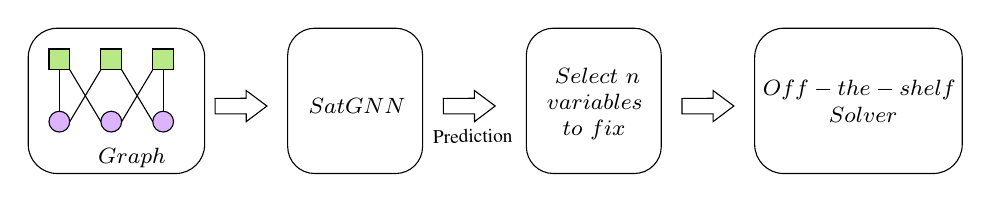
\begin{tikzpicture}[x=0.75pt,y=0.75pt,yscale=-1,xscale=1]
%uncomment if require: \path (0,451); %set diagram left start at 0, and has height of 451

%Shape: Rectangle [id:dp3587479777011455] 
\draw  [fill={rgb, 255:red, 184; green, 233; blue, 134 }  ,fill opacity=1 ] (75,295) -- (85,295) -- (85,305) -- (75,305) -- cycle ;
%Shape: Circle [id:dp623010589573948] 
\draw  [fill={rgb, 255:red, 144; green, 19; blue, 254 }  ,fill opacity=0.32 ] (100,330) .. controls (100,327.24) and (102.24,325) .. (105,325) .. controls (107.76,325) and (110,327.24) .. (110,330) .. controls (110,332.76) and (107.76,335) .. (105,335) .. controls (102.24,335) and (100,332.76) .. (100,330) -- cycle ;
%Shape: Circle [id:dp6210319224354044] 
\draw  [fill={rgb, 255:red, 144; green, 19; blue, 254 }  ,fill opacity=0.32 ] (125,330) .. controls (125,327.24) and (127.24,325) .. (130,325) .. controls (132.76,325) and (135,327.24) .. (135,330) .. controls (135,332.76) and (132.76,335) .. (130,335) .. controls (127.24,335) and (125,332.76) .. (125,330) -- cycle ;
%Shape: Circle [id:dp9356574928412065] 
\draw  [fill={rgb, 255:red, 144; green, 19; blue, 254 }  ,fill opacity=0.32 ] (75,330) .. controls (75,327.24) and (77.24,325) .. (80,325) .. controls (82.76,325) and (85,327.24) .. (85,330) .. controls (85,332.76) and (82.76,335) .. (80,335) .. controls (77.24,335) and (75,332.76) .. (75,330) -- cycle ;
%Shape: Rectangle [id:dp3734262207947956] 
\draw  [fill={rgb, 255:red, 184; green, 233; blue, 134 }  ,fill opacity=1 ] (100,295) -- (110,295) -- (110,305) -- (100,305) -- cycle ;
%Shape: Rectangle [id:dp01885589435556012] 
\draw  [fill={rgb, 255:red, 184; green, 233; blue, 134 }  ,fill opacity=1 ] (125,295) -- (135,295) -- (135,305) -- (125,305) -- cycle ;
%Straight Lines [id:da4907255353964277] 
\draw    (85,305) -- (100,330) ;
%Straight Lines [id:da9596012294566421] 
\draw    (130,305) -- (130,325) ;
%Straight Lines [id:da4248647563144248] 
\draw    (110,305) -- (125,330) ;
%Straight Lines [id:da6077808155610602] 
\draw    (110,330) -- (125,305) ;
%Straight Lines [id:da7849471865454107] 
\draw    (100,305) -- (85,330) ;
%Straight Lines [id:da019130866741998265] 
\draw    (80,305) -- (80,325) ;
%Down Arrow [id:dp06778528901825087] 
\draw   (170.04,330) -- (170.02,326.25) -- (155.03,326.29) -- (155.01,318.79) -- (170,318.75) -- (169.99,315) -- (180.01,322.47) -- cycle ;
%Rounded Rect [id:dp6272397850061886] 
\draw   (65,299) .. controls (65,291.27) and (71.27,285) .. (79,285) -- (136,285) .. controls (143.73,285) and (150,291.27) .. (150,299) -- (150,341) .. controls (150,348.73) and (143.73,355) .. (136,355) -- (79,355) .. controls (71.27,355) and (65,348.73) .. (65,341) -- cycle ;
%Rounded Rect [id:dp6283367026252633] 
\draw   (190,298) .. controls (190,290.82) and (195.82,285) .. (203,285) -- (242,285) .. controls (249.18,285) and (255,290.82) .. (255,298) -- (255,342) .. controls (255,349.18) and (249.18,355) .. (242,355) -- (203,355) .. controls (195.82,355) and (190,349.18) .. (190,342) -- cycle ;
%Rounded Rect [id:dp5504011516450884] 
\draw   (305,298) .. controls (305,290.82) and (310.82,285) .. (318,285) -- (357,285) .. controls (364.18,285) and (370,290.82) .. (370,298) -- (370,342) .. controls (370,349.18) and (364.18,355) .. (357,355) -- (318,355) .. controls (310.82,355) and (305,349.18) .. (305,342) -- cycle ;
%Rounded Rect [id:dp38041408857667824] 
\draw   (415,299) .. controls (415,291.27) and (421.27,285) .. (429,285) -- (501,285) .. controls (508.73,285) and (515,291.27) .. (515,299) -- (515,341) .. controls (515,348.73) and (508.73,355) .. (501,355) -- (429,355) .. controls (421.27,355) and (415,348.73) .. (415,341) -- cycle ;
%Down Arrow [id:dp2151743401001469] 
\draw   (280.01,330) -- (279.99,326.25) -- (265,326.29) -- (264.98,318.79) -- (279.97,318.75) -- (279.96,315) -- (289.98,322.47) -- cycle ;
%Down Arrow [id:dp19599668218528143] 
\draw   (394.99,330) -- (394.98,326.25) -- (379.99,326.29) -- (379.97,318.79) -- (394.96,318.75) -- (394.95,315) -- (404.96,322.47) -- cycle ;

% Text Node
\draw (258.63,332.91) node [anchor=north west][inner sep=0.75pt]  [rotate=-358.87] [align=left] {{\fontfamily{ptm}\selectfont {\scriptsize Prediction}}};
% Text Node
\draw (195,317.4) node [anchor=north west][inner sep=0.75pt]  [font=\footnotesize]  {$~SatGNN$};
% Text Node
\draw (71,341.4) node [anchor=north west][inner sep=0.75pt]  [font=\footnotesize]  {~~~~~~~$Graph$};
% Text Node
\draw (307,301.4) node [anchor=north west][inner sep=0.75pt]  [font=\footnotesize]  {$ \begin{array}{l}
\ Select\ n\ \\
variables\ \\
\ \ to\ fix
\end{array}$};
% Text Node
\draw (411,307.4) node [anchor=north west][inner sep=0.75pt]  [font=\footnotesize]  {$ \begin{array}{c}
Off-the-shelf\ \\
Solver
\end{array}$};


\end{tikzpicture}

}
\caption{Early fixing with SatGNN.}
\label{fig:ef-satgnn}
\end{figure}

Therefore, given a set $\hat{X}$ of random candidate solutions for a given problem instance, we compute \[
\hat{x}^* = \frac{1}{|\hat{X}|}\sum_{\hat{x}\in \hat{X}} \hat{x}\odot \hat{y}(\hat{x}) + (1-\hat{x}) \odot (1 - \hat{y}(\hat{x}))
,\] where $\odot$ is the element-wise product and $\hat{y}(\hat{x})$ is the predicted optimality of candidate solution $\hat{x}\in\hat{X}$ generated using the model from the previous experiment.
In the results reported 

Furthermore, we can say that the closer a given predicted optimal variable $\hat{x}^*_i$ is to 1 (resp. 0), the more certain the model is that that variable should be fixed at 1 (resp. 0).
Therefore, we use the model's certainty to select the variables to be fixed; that is, if we want to fix 50 binary variables, we will choose the 50 variables that the model is most certain of.
We evaluate the accuracy of the SatGNN for early fixing as a function of the number of fixed variables on the two instances of the test set.
These results can be seen in figure \ref{fig:ef-acc}.
As expected, the accuracy decreases as we include variables for which the model is less certain, to the limit of 82.5\% and 87.9\% accuracy on the two instances, which is the accuracy of the predicted optimal solution over the 1745 variables.
A summary of the model's performance when fixing all variables can be seen in Table \ref{tab:exp23-test-performance}.

\begin{figure}[!htb]
    \centering
    \includegraphics[width=0.4\textwidth]{figures/acc_97_9_6.png}
    \includegraphics[width=0.4\textwidth]{figures/acc_97_9_9.png}
    \caption{Early fixing accuracy for the two instances of the ONTS problem in the test set.}
    \label{fig:ef-acc}
\end{figure}

In face of these results, we evaluate how early fixing using SatGNN impacts the optimization performance both in terms of runtime and maximum objective value.
Specifically, we solve the two instances of the ONTS problem on the test set using Gurobi under an increasing number of fixed variables.
The results can be seen in figure \ref{fig:ef-impact}.

\begin{figure}[!htb]
    \centering
    \includegraphics[width=0.4\textwidth]{figures/runtime_obj_97_9_6.png}
    \includegraphics[width=0.4\textwidth]{figures/runtime_obj_97_9_9.png}
    \caption{Optimization results of the two ONTS instances with SatGNN-based early fixing. The objective is plotted with respect to the maximum of the original problem (without any fixed variables). Accuracy is measured with respect to the optimal value of the fixed variables.}
    \label{fig:ef-impact}
\end{figure}

As expected, correctly fixing the variables positively impacts the optimization, while wrongly fixing variables may decrease the runtime but often impacts the objective negatively.
However, we see that, at the limit, a substantial runtime reduction is achieved (90\% and 28\%, for instances 6 and 9, resp.) with a negligible objective cost (1.3\% and 0.3\%, resp.).
Beyond that, fixing more than 500 variables for instance 6 and more than 200 for instance 9 deemed the problems infeasible within a 5 minutes budget.

Given that the SatGNN model could generalize the optimality classification for larger instances of the problem, we also evaluate the impact of early fixing based on our model for the same two larger instances used in the previous experiment.
The performance on the larger instances can be seen in Figure \ref{fig:exp3-larger-instances} and in Table \ref{tab:exp23-test-performance}.
Even though these instances' sizes were not seen during training (not even during validation), the model was still able to handle them and provide sensible early fixing candidates.
The performance drop is significant in terms of accuracy and optimization performance.
In most configurations, however, the model was still able to reduce the runtime with little to no objective value reduction.

\begin{figure}[!htb]
    \centering
    \includegraphics[height=0.3\textwidth]{figures/acc_97_11.png}
    \includegraphics[height=0.3\textwidth]{figures/runtime_obj_97_11.png}
    \includegraphics[height=0.3\textwidth]{figures/acc_120_9.png}
    \includegraphics[height=0.3\textwidth]{figures/runtime_obj_120_9.png}
    \caption{Performance of SatGNN on early fixing instances larger than those seen during training and validation. Instance 97\_11 has 11 jobs, 2 more than the instances previously seen. Instance 120\_9 has the same amount of jobs but schedules for 120-time steps, 23 more than in the instances previously seen.}
    \label{fig:exp3-larger-instances}
\end{figure}

%\subsection{Discussion}

\section{Conclusion}
Throughout the paper, we first analyze the current evaluation methods for diffusion-based adversarial purification and then propose a recommendation for the reliable evaluation of the robustness of adversarial purification. We further investigate the influence of hyperparameters of the diffusion model on the robustness of the purification. Based on our analysis, we propose a new strategy to maximize the benefit of the purification methods.
%\section{Appendix for Proofs}

\paragraph{Proof of Theorem \ref{thm:main}.}

\begin{proof}
\label{proof:main}
Our proof has two steps. In Step 1, we will show that SimCLR is equivalent to minimizing the cross entropy loss defined in Eqn.~(\ref{eqn:cross-entropy}). 
In Step 2, we will show  that minimizing the cross-entropy loss 
is equivalent to spectral clustering on $\bfpi$. 
Combining the two steps together, we have proved our theorem. 

\textbf{Step 1: } SimCLR is equivalent to minimizing the cross entropy loss.

The cross-entropy loss takes expectation over 
$\bfW_\bfX\sim \mathbb{P}(\cdot ; \bfpi)$, 
which means $\bfW_\bfX$ has exactly one non-zero entry in each row $i$. By Lemma~\ref{lem:multinomial}, we know every row $i$ of $\bfW_\bfX$ is independent of other rows. Moreover, 
$\bfW_{\bfX,i}\sim \mathcal{M}(1, \bfpi_i/\sum_j \bfpi_{i,j})=\mathcal{M}(1, \bfpi_i)$, because $\bfpi_i$ itself is a probability distribution.
Similarly, we know $\bfW_\bfZ$ also has the row-independent property by sampling over $\mathbb{P}(\cdot;\bfK_\bfZ)$.
Therefore, by Lemma~\ref{lem:cross_split}, we know Eqn.~(\ref{eqn:cross-entropy}) is equivalent to:
\[
 -\sum_{i=1}^n \mathbb{E}_{\bfW_{\bfX,i}}[\log \mathbb{P}(\bfW_{\bfZ,i}=\bfW_{\bfX,i};\bfK_\bfZ)],
\]

This expression takes expectation over $\bfW_{\bfX,i}$ for the given row $i$. Notice that 
$\bfW_{\bfX,i}$ has exactly one non-zero entry, which equals $1$ (same for $\bfW_{\bfZ,i}$). 
As a result
we expand the above expression to be:
\begin{equation}
 -\sum_{i=1}^n \sum_{j\neq i} \Pr(\bfW_{\bfX,i,j}=1)\log \Pr(\bfW_{\bfZ,i,j}=1).
\label{eqn:detailed-expansion}    
\end{equation}


By Lemma~\ref{lem:multinomial}, $\Pr(\bfW_{\bfZ,i,j}=1)=\bfK_{\bfZ,i,j}/\|\bfK_{\bfZ,i}\|_1$ for $j\neq i$. Recall that $\bfK_\bfZ=(k(\bfZ_i-\bfZ_j))_{(i,j)\in[n]^2}$, which means 
$\bfK_{\bfZ,i,j}/\|\bfK_{\bfZ,i}\|_1=\frac{\exp(-\|\bfZ_i-\bfZ_j\|^2/{2\tau})}{\sum_{k\neq i}
\exp(-\|\bfZ_i-\bfZ_k\|^2/{2\tau})
}$ for $j\neq i$, when $k$ is the Gaussian kernel with variance $\tau$. 

Notice that $\bfZ_i=f(\bfX_i)$, so we know
\begin{equation}
-\log \Pr(\bfW_{\bfZ,i,j}=1)=
-\log \frac{\exp(-\|f(\bfX_i)-f(\bfX_j)\|^2/{2\tau})}{\sum_{k\neq i}
\exp(-\|f(\bfX_i)-f(\bfX_k)\|^2/{2\tau}),
}
\label{eqn:infonce-equivalence}    
\end{equation}


The right hand side is exactly the InfoNCE loss defined in Eqn.~(\ref{eqn:infonce}).
Inserting Eqn.~(\ref{eqn:infonce-equivalence}) into Eqn.~(\ref{eqn:detailed-expansion}), we get the SimCLR algorithm, which first samples augmentation pairs $(i,j)$ with $\Pr(\bfW_{\bfX,i,j}=1)$ for each row $i$, and then optimize the InfoNCE loss. 

\textbf{Step 2: } minimizing the cross entropy loss 
is equivalent to spectral clustering on $\bfpi$.


By Lemma~\ref{lem:convert_to_spectral}, we may further convert the loss to 
\begin{equation}
\label{eqn:main-theorem-repul-attr}
\min_{\bfZ}
-\sum_{(i,j)\in [n]^2} \mathbf{P}_{i,j}
\log k (\bfZ_i-\bfZ_j)+\log \mathbf{R}(\bfZ).
\end{equation}
Since $k$ is the Gaussian kernel, this reduces to \[
\min_\bfZ \mathrm{tr}(\bfZ^\top \mathbf{L}(\bfpi) \bfZ)
+\log \mathbf{R}(\bfZ),
\]

where we use the fact that $\mathbb{E}_{\bfW_\bfX\sim \mathbb{P}(\cdot; \bfpi)}[\mathbf{L}(\bfW_\bfX)]
=\mathbf{L}(\bfpi)
$, because the Laplacian operator is linear and $
\mathbb{E}_{\bfW_\bfX\sim \mathbb{P}(\cdot; \bfpi)}(\bfW_\bfX)=\bfpi
$.
\end{proof}

\paragraph{Proof of Theorem \ref{thm:clip}.}
\begin{proof}
Since $\bfW_\bfX\sim \mathbb{P}(\cdot;\bfpi_{\mathbf{A}, \mathbf{B}})$, we know 
$\bfW_\bfX$ has exactly one non-zero entry in each row, denoting the pair that got sampled. 
A notable difference compared to the previous proof is we now have $n_\mathcal{A}+n_\mathcal{B}$ objects in our graph. CLIP deals with this by taking a mini-batch of size $2N$, 
such that $n_\mathcal{A}=n_\mathcal{B}=N$, and adding the $2N$ InfoNCE losses together. We label the objects in $\mathcal{A}$ as $[n_\mathcal{A}]$, and the objects in $\mathcal{B}$ as $\{n_\mathcal{A}+1, \cdots, n_\mathcal{A}+n_\mathcal{B}\}$. 

Notice that $\bfpi_{\mathbf{A}, \mathbf{B}}$ is a bipartite graph, so the edges of objects in $\mathcal{A}$ will only connect to object in $\mathcal{B}$ and vice versa. We can define the similarity matrix in $\cZ$ as $\bfK_\bfZ$, 
where $\bfK_\bfZ(i, j+n_\mathcal{A})=\bfK_\bfZ(j+n_\mathcal{A},i)= k(\bfZ_i-\bfZ_j)$ for $i\in [n_\mathcal{A}], j\in [n_\mathcal{B}]$, and otherwise we set $\bfK_\bfZ(i,j)=0$. 
The rest is same as the previous proof. 
\end{proof}

\paragraph{Proof of Theorem \ref{thm:exponential}.}

\begin{proof}
\label{proof:exponential}
Since the objective function consists of a linear term combined with an entropy regularization, which is a strongly concave function, the maximization problem is a convex optimization problem. Owing to the implicit constraints provided by the entropy function, the problem is equivalent to having only the equality constraint. We then introduce the Lagrangian multiplier $\lambda$ and obtain the following relaxed problem:

$$
\widetilde{E}(\boldsymbol{\alpha})=\psi_{1}-\sum_{i=1}^n \alpha_{i} \psi_{i}+\tau \sum_{i=1}^n \alpha_{i}\log \alpha_{i}+\lambda\left(\boldsymbol{\alpha}^{\top} \mathbf{1}_n-1\right).
$$

As the relaxed problem is unconstrained, taking the derivative with respect to $\alpha_{i}$ yields

$$
\frac{\partial \widetilde{E}(\boldsymbol{\alpha})}{\partial \alpha_{i}}=-\psi_{i}+\tau\left(\log \alpha_{i}+\alpha_{i} \frac{1}{\alpha_{i}}\right)+\lambda=0.
$$

Solving the above equation implies that $\alpha_{i}$ takes the form
$
\alpha_{i}=\exp \left(\frac{1}{\tau} \psi_{i}\right) \exp \left(\frac{-\lambda}{\tau}-1\right).
$ Since $\alpha_{i}$ lies on the probability simplex, the optimal $\alpha_{i}$ is explicitly given by
$
\alpha^{*}_{i}=\frac{\exp \left(\frac{1}{\tau} \psi_{i}\right)}{\sum_{i^{\prime}=1}^n \exp \left(\frac{1}{\tau} \psi_{i^{\prime}}\right)} .
$ Substituting the optimal point into the objective function, we obtain
$$
\begin{aligned}
E\left(\boldsymbol{\alpha}^*\right)  &=\psi_1-\sum_{i=1}^n \frac{\exp \left(\frac{1}{\tau} \psi_{i}\right)}{\sum_{i^{\prime}=1}^n \exp \left(\frac{1}{\tau} \psi_{i^{\prime}}\right)} \psi_{i}+\tau \sum_{i=1}^n \frac{\exp \left(\frac{1}{\tau} \psi_{i}\right)}{\sum_{i^{\prime}=1}^n \exp \left(\frac{1}{\tau} \psi_{i^{\prime}}\right)}\log \frac{\exp \left(\frac{1}{\tau} \psi_{i}\right)}{\sum_{i^{\prime}=1}^n \exp \left(\frac{1}{\tau} \psi_{i^{\prime}}\right)} \\
& =\psi_1 - \tau \log \left(\sum_{i=1}^n \exp \left(\frac{1}{\tau} \psi_{i}\right)\right).
\end{aligned}
$$
Thus, the Lagrangian dual function is given by
\begin{equation*}
-E\left(\boldsymbol{\alpha}^*\right)= -\tau \log \frac{\exp \left(\frac{1}{\tau} \psi_{1}\right)}{\sum_{i=1}^n \exp \left(\frac{1}{\tau} \psi_{i}\right)}.\qedhere
\end{equation*}
\end{proof}



\section{More on Experiments} \label{section: experiment_details}

\paragraph{CIFAR-10 and CIFAR-100} CIFAR-10 ~\citep{krizhevsky2009learning} and CIFAR-100 ~\citep{krizhevsky2009learning} are well-known classic image classification datasets. Both CIFAR-10 and CIFAR-100 contain a total of 60k $32 \times 32$ labeled images of different classes, with 50k for training and 10k for testing. CIFAR-10 is similar to CIFAR-100, except there are 10 different classes in CIFAR-10 and 100 classes in CIFAR-100.

\paragraph{TinyImageNet} TinyImageNet ~\citep{le2015tiny} is a subset of ImageNet ~\citep{deng2009imagenet}. There are 200 different object classes in TinyImageNet, with 500 training images, 50 validation images, and 50 test images for each class. All the images in TinyImageNet are colored and labeled with a size of $64 \times 64$.

\textbf{Pseudo-code.} Algorithm \ref{alg:Training Procedure} presents the pseudo-code for our empirical training procedure.

\begin{algorithm}[!htbp]
\caption{Training Procedure}
\label{alg:Training Procedure}
\begin{algorithmic}[1]
\REQUIRE trainable encoder network $f$, batch size $N$, augmentation strategy \textit{aug}, loss function $L$ with hyperparameters \textit{args}
\FOR {sampled minibatch ${x_i}_{i=1}^N$}
\FORALL{$i \in { 1, ..., N }$}
\STATE draw two augmentations $t_i = \textit{aug}\left(x_i\right) $, $t_i' = \textit{aug}\left(x_i\right) $
\STATE $z_i = f\left(t_i\right)$, $z_i' = f\left(t_i'\right)$
\ENDFOR
\STATE compute loss $\mathcal{L} = L(N, z, z', \textit{args})$
\STATE update encoder network $f$ to minimize $\mathcal{L}$
\ENDFOR
\STATE \textbf{Return} encoder network $f$
\end{algorithmic}
\end{algorithm}

We also provide the pseudo-code for our core loss function used in the training procedure in Algorithm \ref{alg:Core loss}. The pseudo-code is almost identical to SimCLR's loss function, with the exception of an extra parameter $\gamma$.

\begin{algorithm}[!htbp]
\caption{Core loss function $\mathcal{C}$}
\label{alg:Core loss}
\begin{algorithmic}[1]
\REQUIRE batch size $N$, two encoded minibatches $z_1, z_2$, $\gamma$, temperature $\tau$
\STATE $z = \textit{concat}\left(z_1, z_2\right)$
\FOR {$i \in {1, ..., 2N }, j \in {1, ..., 2N}$ }
\STATE $s_{i,j} = \Vert z_i - z_j \Vert_2^{\gamma}$
\ENDFOR
\STATE \textbf{define} $l(i, j)$ \textbf{as} $l(i, j) = - \log \frac{exp\left(s_{i,j}/\tau \right)}{\sum_{k=1}^{2N} \mathbf{1}{[k \ne i]} exp\left(s{i, j} / \tau \right)} $
\STATE \textbf{Return} $\frac{1}{2N} \sum_{k=1}^N\left[l(i, i+N) + l(i+N, i)\right]$
\end{algorithmic}
\end{algorithm}

Utilizing the core loss function $\mathcal{C}$, we can define all kernel loss functions used in our experiments in Table \ref{table: loss definition}. For all $z_i \in z$ with even dimensions $n$, we define $z_{L_i} = z_i\left[0:n/2\right]$ and $z_{R_i} = z_i\left[n/2:n\right]$.

\begin{table}[ht]
\centering
\begin{tabular}{{@{}l|l@{}}}
Kernel  &  Loss function \\ \midrule
Laplacian & $\mathcal{C}\left(N, z, z', \gamma=1, \tau\right)$\\ \midrule
Sum       & $\lambda * \mathcal{C}\left(N, z, z', \gamma=1, \tau_1\right) + (1-\lambda) * \mathcal{C}\left(N, z, z', \gamma=2, \tau_2\right)$  \\ \midrule
Concatenation Sum&$\lambda * \mathcal{C}\left(N, z_L, z'_L, \gamma=1, \tau_1\right) + (1-\lambda) * \mathcal{C}\left(N, z_R, z'_R, \gamma=2, \tau_2\right)$\\ \midrule
$\gamma = 0.5$ & $\mathcal{C}\left(N, z, z', \gamma=0.5, \tau\right)$          \\ 

\end{tabular}

\caption{Definition of kernel loss functions in our experiments}
\label {table: loss definition}
\end{table}

\textbf{Baselines.} We reproduce the SimCLR algorithm using PyTorch Lightning~\citep{PytorchLightning}.

\textbf{Encoder details.}
The encoder $f$ consists of a backbone network and a projection network. We employ ResNet50~\citep{ResNet} as the backbone and a 2-layer MLP (connected by a batch normalization~\citep{ioffe2015batch} layer and a ReLU \cite{nair2010rectified} layer) with hidden dimensions 2048 and output dimensions 128 (or 256 in the concatenation kernel case).

\textbf{Encoder hyperparameter tuning.}
For each encoder training case, we randomly sample 500 hyperparameter groups (sample details are shown in Table \ref{table: Hyperparameter sample}) and train these samples simultaneously using Ray Tune ~\citep{RayTune}, with the ASHA scheduler~\citep{li2018massively}. Ultimately, the hyperparameter group that maximizes the online validation accuracy (integrated in PyTorch Lightning) within 5000 validation steps is chosen for the given encoder training case.

\begin{table}[ht]
\centering

\begin{tabular}{@{}l|l|l@{}}
\midrule
Hyperparameter  & Sample Range & Sample Strategy \\ \midrule
start learning rate & $\left[10^{-2}, 10\right]$ & log uniform \\ \midrule
$\lambda$       & $\left[0, 1\right]$ & uniform \\ \midrule
$\tau$, $\tau_1$, $\tau_2$ & $\left[0, 1\right]$ & log uniform \\ \midrule
\end{tabular}

\caption{Hyperparameters sample strategy}
\label {table: Hyperparameter sample}
\end{table}

\textbf{Encoder training.} 
We train each encoder using the LARS optimizer~\citep{LARSOptimizer}, LambdaLR Scheduler in PyTorch, momentum 0.9, weight decay $10^{-6}$, batch size 256, and the aforementioned hyperparameters for 400 epochs on a single A-100 GPU.

\textbf{Image transformation.} The image transformation strategy, including augmentation, is identical to the default transformation strategy provided by PyTorch Lightning.

\textbf{Linear evaluation.}
The linear head is trained using the SGD optimizer with a cosine learning rate scheduler, batch size 64, and weight decay $10^{-6}$ for 100 epochs. The learning rate starts at $0.3$ and ends at $0$.

\textbf{Moco Experiments.} We also tested our method based on MoCo~\citep{he2019moco}. The results are summarized in Table \ref{tab:results-moco}. Here we choose ResNet18~\citep{ResNet} as the backbone and set a temperature of $0.1$ as default. For our simple sum kernel, we set $\lambda=0.8$. The results show that our method outperforms the original MoCo method.

\begin{table}[thb]
\centering
\caption{MoCo Experiment Results on CIFAR-10 and CIFAR-100.}
\label{tab:results-moco}
\resizebox{\textwidth}{!}{%
\begin{tabular}{@{}c|ccc|ccc@{}}
\toprule
\multirow{3}{*}{Method} & \multicolumn{3}{c|}{CIFAR-10} & \multicolumn{3}{c}{CIFAR-100} \\ \cmidrule(lr){2-4} \cmidrule(lr){5-7} 
                        & 200 epochs & 400 epochs    & 1000 epochs   & 200 epochs & 400 epochs & 1000 epochs         \\ \midrule
MoCo (repro.)         & $76.41 \pm 0.12$    & $80.01 \pm 0.15$          & $84.45 \pm 0.08$    & $\mathbf{47.02 \pm 0.11}$ & $52.50 \pm 0.07$ & $57.62 \pm 0.15$            \\
\midrule
Laplacian Kernel        & ${78.09 \pm 0.10}$    & $\mathbf{83.85 \pm 0.09}$          & $\mathbf{88.34 \pm 0.16}$    & $46.12 \pm 0.22$   & $53.44 \pm 0.17$ & $59.10 \pm 0.14$        \\
Simple Sum Kernel & $\mathbf{78.12 \pm 0.15}$   & $83.23 \pm 0.18$ & $87.50 \pm 0.20$ & $46.65 \pm 0.06$ & $\mathbf{53.62 \pm 0.19}$ & $\mathbf{59.83 \pm 0.12}$\\
\bottomrule
\end{tabular}
}
\end{table}



\section{More Experiments on Synthetic Data}


Consider a scenario with $n$ clusters, each containing $k$ vertices. Let the probability of vertices $u$ and $v$ from the same cluster belonging to $\bfpi$ be $p$. Conversely, for vertices $u$ and $v$ from different clusters, let the probability of belonging to $\pi$ be $q$. We generate the graph $\bfpi$ randomly, based on $p$ and $q$. We experiment with values of $k=100$ and $n=6$ for ease of visualization, embedding all points in a two-dimensional space. Each vertex's initial position originates from a normal distribution. In each iteration, we sample a subgraph of $\bfpi$ uniformly, ensuring each vertex has an out-degree of $1$. We then optimize the corresponding vectors using InfoNCE loss with an SGD optimizer and iterate until convergence. Our experimental setup consists of an SGD learning rate of $1$, an InfoNCE loss temperature of $0.5$, and a batch size of $50$. We evaluate two scenarios with different $p$ and $q$ values: $p=1$, $q=0$, and $p=0.75$, $q=0.2$. The results of these experiments are visualized in Figure \ref{fig:vis-spectral-cluster}. The obtained embeddings exhibit the hallmark pattern of spectral clustering of graph $\bfpi$.

\begin{figure}[!tb]
\centering
\subfigure{
\includegraphics[width=1\textwidth]{Figures/cluster_pi.png}
\label{fig:vis-cluster}
}
\subfigure{
\includegraphics[width=1\textwidth]{Figures/noised_cluster_pi.png}
\label{fig:vis-noised-cluster}
}
\caption{Visualizations of the optimization process using InfoNCE Loss on the vectors corresponding to $\bfpi$. Points of identical color belong to the same cluster within $\bfpi$. To showcase the internal structure of $\bfpi$, we randomly select 10 vertices from each cluster to display the edge distribution of $\bfpi$.}
\label{fig:vis-spectral-cluster}
\end{figure}



\section*{Acknowledgments}

The authors acknowledge support from CNPq (Conselho Nacional de Desenvolvimento Cient{\'\i}fico e Tecnol{\'o}gico) under grant number 150281/2022-6, 404576/2021-4 as well as FAPESC under grant number 2021TR001851. 




%\begin{figure}[t]
%\includegraphics{}
%\caption{Figure caption.}\label{f1}
%\end{figure}

%\begin{table*}
%\caption{} \label{t1}
%\begin{tabular}{lll}
%\hline
%&&\\
%&&\\
%\hline
%\end{tabular}
%\end{table*}


%%%%%%%%%%% The bibliography starts:
%\bibliographystyle{ieeetr}


%\bibliographystyle{elsarticle-harv}
\bibliographystyle{ieeetr}
%\biboptions{authoryear}
\bibliography{main.bib}

\end{document}

